\documentclass{fast-nuces-bs}
%\documentclass{article}

% ---------------------------------------------------------------------------
% FlakeTrace — FYP-1 Mid Report (F26-214)
% Owner of this file: M2 (Abdul Raffay). Other members: change it only by PR.
% Rules for editing the report: mid-eval-report/CLAUDE.md
% ---------------------------------------------------------------------------

\usepackage{blindtext}
\usepackage{mathptmx}% Times Roman font
\usepackage[T1]{fontenc}
\usepackage{lipsum}
\usepackage{sectsty}
\usepackage{tikz-uml}
\usepackage{titlesec}

% Added for FlakeTrace: the template's chapters use longtable/booktabs but did not load them.
\usepackage{booktabs}
\usepackage{longtable}
\usepackage{array}
\usepackage{float}
\usepackage{xcolor}
\usepackage{listings}
% Long \texttt file names cannot hyphenate; let LaTeX stretch spaces instead of overflowing the margin.
\setlength{\emergencystretch}{3em}
% The class loads natbib in author-year mode; IEEEtran is numeric, so citations fail without this.
\setcitestyle{numbers,square}
% \pr{49} prints a clickable "#49" linking to that pull request.
\newcommand{\pr}[1]{\href{https://github.com/zoyaahmad428/FlakeTrace/pull/#1}{\##1}}

% Marks unfinished text. CI does not fail on it, but the final PDF must contain none:
%   grep -rn '\\todo{' chapters/   must print nothing before submission.
\newcommand{\todo}[1]{\textcolor{red}{\textbf{[TODO: #1]}}}

% A figure slot that can be cited before the diagram exists.
% Usage: \placeholderfig{ch5:fig:arch}{Caption text}{M2}
% Replace with a real \includegraphics figure; keep the same label and caption.
\newcommand{\placeholderfig}[3]{%
  \begin{figure}[H]\centering
    \fbox{\parbox[c][4cm][c]{0.8\textwidth}{\centering\textcolor{red}{\textbf{Diagram pending (#3)}}}}
    \caption{#2}\label{#1}
  \end{figure}}

% Used by chapters/01_students_submission.tex (the template referenced these but never defined them)
\newcommand{\projecttitle}{FlakeTrace: Evidence-Certified Diagnosis of Order-Dependent Java Test Failures}
\newcommand{\studentone}{Zoya Ahmad (23i-0805)}
\newcommand{\studenttwo}{Abdul Raffay (23i-0587)}
\newcommand{\studentthree}{Zarpash Nasim (23i-0027)}

% Information about the Thesis
% -----------------------------------------------------------------------------
% (All are compulsory, do not delete any line other than author Information)
% For e.g., usually there are 3 students in a group, so leave authorone,
% authortwo, and authorthree, and delete authorfour.
%%%%%%%%%%%%%%%%%%%%%%%%%%%%%%%%%%%%%%%%%%%%%%%%%%%%%%%%%%%%%%%%%%%%%%%%%%%%%%%
\department{FAST School of Computing}
\faculty{Computer Science}
\degreeyear{2026}
\degreemonth{October}
\degreename{Computer Science}
\campuscity{Islamabad}
\authorone{Zoya Ahmad}{23i-0805}
\authortwo{Abdul Raffay}{23i-0587}
\authorthree{Zarpash Nasim}{23i-0027}
\supervisor{TODO: Supervisor Name}
\sessionduration{2023-2027}
% Uncomment only if there is a co-supervisor (the title page changes layout when it is set):
%\cosupervisor{Mr./ Ms./ Dr. Co-Supervisor Name}
\deanname{Dr. Dean Computing}
\directorname{Dr. Director of the Campus}
\hodname{Dr. Head of Computer Science Department}
\fypcoordinatorname{Name of FYP Coordinator}
\title{\projecttitle}
%%%%%%%%%%%%%%%%%%%%%%%%%%%%%%%%%%%%%%%%%%%%%%%%%%%%%%%%%%%%%%%%%%%%%%%%%%%%%%%

%%%%%%%%%%%%%%%%%%%%%%%%%%%%%%%%%%%%%%%%%%%%%%%%%%%%%%%%%%%%%%%%%%%%%%%%%%%%%%
% Former document starts below this
\begin{document}

\cleardoublepage
\pagenumbering{roman}
% ===========================================================================
% OWNER: M2 (Abdul Raffay)
% GRADED BY: Form 3 #1 Format (signatures required)
% DRAW FROM: main.tex macros
% Rules: mid-eval-report/CLAUDE.md. Do not edit a file you do not own.
% ===========================================================================
\chapter*{Students' Submission}
\addcontentsline{toc}{chapter}{Students' Submission}
We certify that this report is submitted as the FYP-1 mid-report for the project titled \textit{\projecttitle}.
\vspace{1cm}
\begin{tabular}{p{0.45\textwidth}p{0.45\textwidth}}
Student 1: \studentone & Signature: \rule{0.25\textwidth}{0.4pt}\\[1cm]
Student 2: \studenttwo & Signature: \rule{0.25\textwidth}{0.4pt}\\[1cm]
Student 3: \studentthree & Signature: \rule{0.25\textwidth}{0.4pt}
\end{tabular}

% ===========================================================================
% OWNER: M2 (Abdul Raffay)
% GRADED BY: Form 3 #1 Format
% DRAW FROM: template text, keep as is
% Rules: mid-eval-report/CLAUDE.md. Do not edit a file you do not own.
% ===========================================================================
\chapter*{Anti-Plagiarism Statement}
\addcontentsline{toc}{chapter}{Anti-Plagiarism Statement}
The students certify that this report is their own work and that all sources used in preparing the report have been appropriately acknowledged and referenced.

% ===========================================================================
% OWNER: M2 (Abdul Raffay)
% GRADED BY: Form 3 #1 Format
% DRAW FROM: template text, keep as is
% Rules: mid-eval-report/CLAUDE.md. Do not edit a file you do not own.
% ===========================================================================
\chapter*{Authors' Declaration}
\addcontentsline{toc}{chapter}{Authors' Declaration}
We declare that the work documented in this report represents the work completed by the project team up to the FYP-1 mid-report stage. Contributions, tools, external components, and relevant sources are disclosed where applicable.

% ===========================================================================
% OWNER: JOINT, written LAST (M2 assembles, all three approve)
% GRADED BY: Form 3 #1-#3
% DRAW FROM: finished chapters 1-10 only
% NOTE: 150-200 words: problem, method, key results (real numbers from ch8), conclusion
% Rules: mid-eval-report/CLAUDE.md. Do not edit a file you do not own.
% ===========================================================================
\chapter*{Abstract}
\addcontentsline{toc}{chapter}{Abstract}
When a Java test passes on its own but fails after other tests, developers can see the instability but have no bounded, checkable way to find which earlier test caused it and why. FlakeTrace is a self-hosted command-line tool that diagnoses one such order-dependent failure in a Maven project. It reproduces the failure, checks the failing test alone, finds the responsible tests through controlled reruns and delta debugging, repeats the reduced order twenty times with a 95\% Wilson interval, and names the shared static field or system property with the exact bytecode locations where it is written and read, without changing the project. When the evidence is insufficient it refuses with a typed reason instead of guessing. Iteration 1 implements this path in one command. On a seeded fixture, all four order-dependent cases were verified, reproducing 20 of 20 times and never alone, and all three negative controls ended unresolved with a typed reason. The evidence extractor has also been run on one real project, fastjson. Iteration 2 and FYP-2 add candidate ranking, an execution budget, runtime evidence, a container and evaluation against published baselines on real projects.

% ===========================================================================
% OWNER: M2 (Abdul Raffay)
% GRADED BY: Form 3 #1 Format
% DRAW FROM: -
% Rules: mid-eval-report/CLAUDE.md. Do not edit a file you do not own.
% ===========================================================================
\chapter*{Acknowledgments}
\addcontentsline{toc}{chapter}{Acknowledgments}
We thank our supervisor, Dr. Ali Zeeshan, for the guidance given to us throughout this project. We also thank the members of the proposal defence panel: their questions, how the system works without logs, whether code is injected or modified, how the failing code is isolated and where the approach applies, set the direction of this first iteration. Finally, we thank the faculty of the FAST School of Computing, Islamabad, for their support.

% ===========================================================================
% OWNER: JOINT, written LAST (M2 assembles, all three approve)
% GRADED BY: Form 3 #1-#3
% DRAW FROM: finished chapters; docs/00-Meta/project-one-pager.md
% Rules: mid-eval-report/CLAUDE.md. Do not edit a file you do not own.
% ===========================================================================
\chapter*{Executive Summary}
\addcontentsline{toc}{chapter}{Executive Summary}
Provide a one- to two-page overview of the project, motivation, scope, research findings, current implementation, validation status, risks, and remaining work.

\tableofcontents
\listoffigures
\listoftables
% ===========================================================================
% OWNER: M2 (Abdul Raffay) - others request additions in their PR description
% GRADED BY: Form 3 #1 Format
% DRAW FROM: docs/00-Meta/glossary.md
% Rules: mid-eval-report/CLAUDE.md. Do not edit a file you do not own.
% ===========================================================================
\chapter*{List of Abbreviations}
\addcontentsline{toc}{chapter}{List of Abbreviations}
% Every abbreviation below appears in at least one chapter (checked with grep on 11 October 2026).
% Members: request additions in your pull-request description.
\begin{longtable}{@{}p{0.18\textwidth}p{0.72\textwidth}@{}}
ADR & Architecture Decision Record\\
AI & Artificial Intelligence\\
CDR & Certificate-Driven Remediation (gated module, FYP-2)\\
CI & Continuous Integration\\
CLI & Command-Line Interface\\
FR & Functional Requirement\\
FYP & Final Year Project\\
GenAI & Generative Artificial Intelligence\\
ID & Identifier\\
JDK & Java Development Kit\\
JSON & JavaScript Object Notation\\
JVM & Java Virtual Machine\\
NFR & Non-Functional Requirement\\
OD & Order-Dependent (test)\\
OS & Operating System\\
PDF & Portable Document Format\\
PID & Process Identifier\\
POC & Proof of Concept\\
PR & Pull Request\\
SHA & Secure Hash Algorithm (SHA-256 for file hashes; also a git commit hash)\\
SSH & Secure Shell\\
UC & Use Case\\
UML & Unified Modeling Language\\
WP & Work Package\\
WSL & Windows Subsystem for Linux\\
\end{longtable}


\cleardoublepage
\pagenumbering{arabic}
% ===========================================================================
% OWNER: M1 (Zoya Ahmad)
% GRADED BY: Form 3 #3 Vision, scope & success criteria (10)
% DRAW FROM: docs/00-Meta/project-one-pager.md, docs/02-Requirements/scope-boundary.md, docs/00-Meta/stream-and-status.md, docs/00-Meta/stakeholder-evidence.md, docs/07-Defense/decisions/*
% NOTE: Scope must match the approved proposal and the post-defence narrowing; success criteria must be measurable
% Rules: mid-eval-report/CLAUDE.md. Do not edit a file you do not own.
% ===========================================================================
\chapter{Introduction and Project Vision}
\section{Project Overview}
Describe the product/application/system and its intended purpose.
\section{Problem Statement}
Clearly formulate the problem being addressed.
\section{Problem Context and Motivation}
Explain the context, stakeholders, motivation, and significance.
\section{Project Vision}
State what the project intends to achieve.
\section{Project Objectives}
List measurable project objectives.
\section{Project Scope}
Define included and excluded functionality.
\section{Project Modules}
Describe the major modules and their responsibilities.
\section{Stakeholders and User Classes}
Identify users, stakeholders, and their characteristics.
\section{Success Criteria}
Define measurable criteria that will indicate project success.
\section{Constraints and Assumptions}
Document relevant constraints and assumptions.
\section{Ethical, Legal and DEI Considerations}
Document relevant ethical, legal, accessibility, privacy, or diversity considerations where applicable.

% ===========================================================================
% OWNER: M1 (Zoya Ahmad)
% GRADED BY: Form 3 #2 Problem, R&D & gap analysis (15) - red flag: generic/AI-summarised text
% DRAW FROM: docs/01-Literature/* (per-paper notes, contemporary-comparison-table.md, commercial-tools.md, prior-fyp-comparison.md, references.md), docs/05-Testing/poc/*
% NOTE: Cite only papers a member has opened. Put BibTeX in references/refs-m1.bib
% Rules: mid-eval-report/CLAUDE.md. Do not edit a file you do not own.
% ===========================================================================
\chapter{Research and Existing Solutions}
\section{Research Method / Approach}
Describe how relevant technical and domain knowledge was investigated.
\section{Existing Solutions / Products}
Review relevant existing solutions.
\section{Comparison of Existing Solutions}
Compare solutions using project-relevant criteria.
\section{Limitations and Gaps}
Identify limitations and the gap motivating the proposed solution.
\section{Proposed Solution}
Explain how the proposed system addresses the identified gap.
\section{Complex Computing Problem}
Clearly identify and explain the complex computing problem addressed by the project.
\section{Technical Challenges}
Document major technical challenges anticipated or encountered.
\section{Research Findings and Design Decisions}
Explain how research findings influenced requirements, architecture, algorithms, tools, or other decisions.

% ===========================================================================
% OWNER: M2 (Abdul Raffay)
% GRADED BY: Form 2 #1-#2 (panel actions, iteration plan); Form 3 #1
% DRAW FROM: docs/08-MidEval/panel-action-register.md, docs/08-MidEval/iteration-plan.md, docs/00-Meta/roadmap.md, docs/09-Team/members.md, Mid Eval/FlakeTrace-Defense.pdf (summarised in panel-action-register.md)
% NOTE: Every action in the register appears here, including open ones, each with an evidence link
% Rules: mid-eval-report/CLAUDE.md. Do not edit a file you do not own.
% ===========================================================================
\chapter{Proposal Feedback and Iteration Plan}
\section{Proposal Feedback Summary}\label{ch3:sec:feedback}
The proposal was defended on 11 September 2026 and the decision was \textbf{Approved with Minor Modifications}. The panel wrote:
\begin{quote}
Approved. Do more research to improve your proposed solution and implement the given suggestions. \ldots{} students need to think more carefully about the proposed solution (e.g., in the case of a Flake Trace, how will the system detect it if no logs are available?). In the next presentation, students need to answer: 1) Will log trace instructions be injected into the code? 2) Will the code be modified? 3) How will the code block be isolated? 4) What are diverse scenarios where this approach is applicable?
\end{quote}
We turned each point into a numbered action, A1--A6, and added four actions, A7--A10, from sections 7--10 of the post-defence improvement and execution plan (\path{Mid Eval/FlakeTrace-Defense.pdf}). Every action has an owner, a decision, a status and an evidence link, kept in \path{docs/08-MidEval/panel-action-register.md} and updated whenever the work moved it.

\section{Proposal Action Register}\label{ch3:sec:register}
Table~\ref{ch3:tab:register} summarises all ten actions; Appendix~\ref{app:action-register} gives each one in full with every evidence path. Links are to the pull requests that closed them.

{\small
\begin{longtable}{>{\raggedright\arraybackslash}p{0.05\textwidth}>{\raggedright\arraybackslash}p{0.27\textwidth}>{\raggedright\arraybackslash}p{0.30\textwidth}>{\raggedright\arraybackslash}p{0.12\textwidth}>{\raggedright\arraybackslash}p{0.12\textwidth}}
\caption{Proposal action register (summary)}\label{ch3:tab:register}\\
\toprule
No. & Feedback / required change & Action taken & Status & Evidence\\
\midrule
\endfirsthead
\toprule
No. & Feedback / required change & Action taken & Status & Evidence\\
\midrule
\endhead
A1 & How will it detect the problem with no logs? & Detection uses only test order, pass/fail, exceptions and stack traces from re-execution, plus bytecode evidence; the fixture has no logging & Complete & \pr{26}, \pr{35}, \pr{49}\\
A2 & Will trace instructions be injected? & No: evidence is read from compiled classes with \texttt{javap}; nothing is injected (ADR-001) & Complete & \pr{9}, \pr{15}\\
A3 & Will the code be modified? & No: every project file is hashed before and after; a change forces \texttt{UNRESOLVED} & Complete & \pr{11}\\
A4 & How will the code block be isolated? & Sequence isolation (alone check, polluter search, \texttt{ddmin}, repeated runs) and cause localisation (resource with bytecode offsets) & Complete & \pr{11}, \pr{15}, \pr{34}, \pr{35}\\
A5 & Which diverse scenarios apply? & Seven fixture cases, including two polluters, a needed reorder and three negative controls; unsupported causes reported as \texttt{UNRESOLVED} & Complete & \pr{45}, \pr{49}\\
A6 & Do more research to improve the solution & Research note on one-by-one search versus \texttt{ddmin}; measured over-approximation added to ADR-001 & Complete & \pr{50}\\
A7 & Record the controlled execution environment & Execution record per run with JDK, OS, project commit, uncommitted changes and shuffle seeds; no container yet & Complete & \pr{41}, \pr{49}\\
A8 & Reproduction confidence & $n$ repeats, victim-alone comparison and Wilson interval in every real report & Complete & \pr{57}\\
A9 & An evidence report with all fields & Schema-validated reports for all seven fixture cases, produced by the real pipeline & Complete & \pr{57}\\
A10 & The plan lists databases, ports, threads, caches & Adapted: Iteration 1 keeps static fields and system properties, filesystem paths in Iteration 2; others reported as unsupported & Decided; supervisor confirmation pending & ---\\
\bottomrule
\end{longtable}}

Nine actions are complete. A10 is a scope decision that we will ask the supervisor to confirm at the Mid evaluation; until then it is not counted as closed.
\section{Iteration Strategy}
Describe the iterative development strategy.
\section{Iteration 1 Plan}
Define objectives, selected features, deliverables, and evidence.
\section{Iteration 2 Plan}
Define objectives, selected features, deliverables, and evidence.
\section{Work Breakdown and Responsibilities}
Describe task allocation and ownership.
\section{Progress Against Plan}
Compare planned milestones with actual progress.
% Planned-vs-actual Gantt (M2): diagrams/m2/gantt.puml -> figures/m2/gantt.png
\placeholderfig{ch3:fig:gantt}{Iteration 1: planned versus actual schedule}{M2}
\section{Delays, Deviations and Recovery Plan}
Explain deviations and recovery actions.

% ===========================================================================
% OWNER: M3 (Zarpash Nasim)
% GRADED BY: Form 3 #4 Requirements & acceptance criteria (15)
% DRAW FROM: docs/02-Requirements/functional.md, non-functional.md, scope-boundary.md, docs/03-Design/certificate-contract.md, eval/schema/report.schema.json, fixtures/od-fixture/ground_truth.json
% NOTE: Every FR/NFR needs an objective acceptance check; the traceability table links FR -> module -> file -> test
% Rules: mid-eval-report/CLAUDE.md. Do not edit a file you do not own.
% ===========================================================================
\chapter{Software Requirements}
\section{User Interactions / Use Cases}
FlakeTrace has two actors. A \textbf{Developer} invokes it directly against a failing test
they are investigating. A \textbf{CI Pipeline} invokes it the same way, on demand for a known
failing test rather than on every build --- Non-Functional Requirement NFR-1 (Section
\ref{ch4:sec:nfr}) is the reason: our stakeholders' own CI-time budgets rule out running it on
every successful build. Both actors drive the same seven use cases (Figure
\ref{ch4:fig:usecases}): submit a diagnosis request, through to receiving a typed certificate.

\section{Use Case Diagram}
% Use case diagram (M3): diagrams/m3/use_cases.puml -> figures/m3/use_cases.png
\begin{figure}[H]\centering
  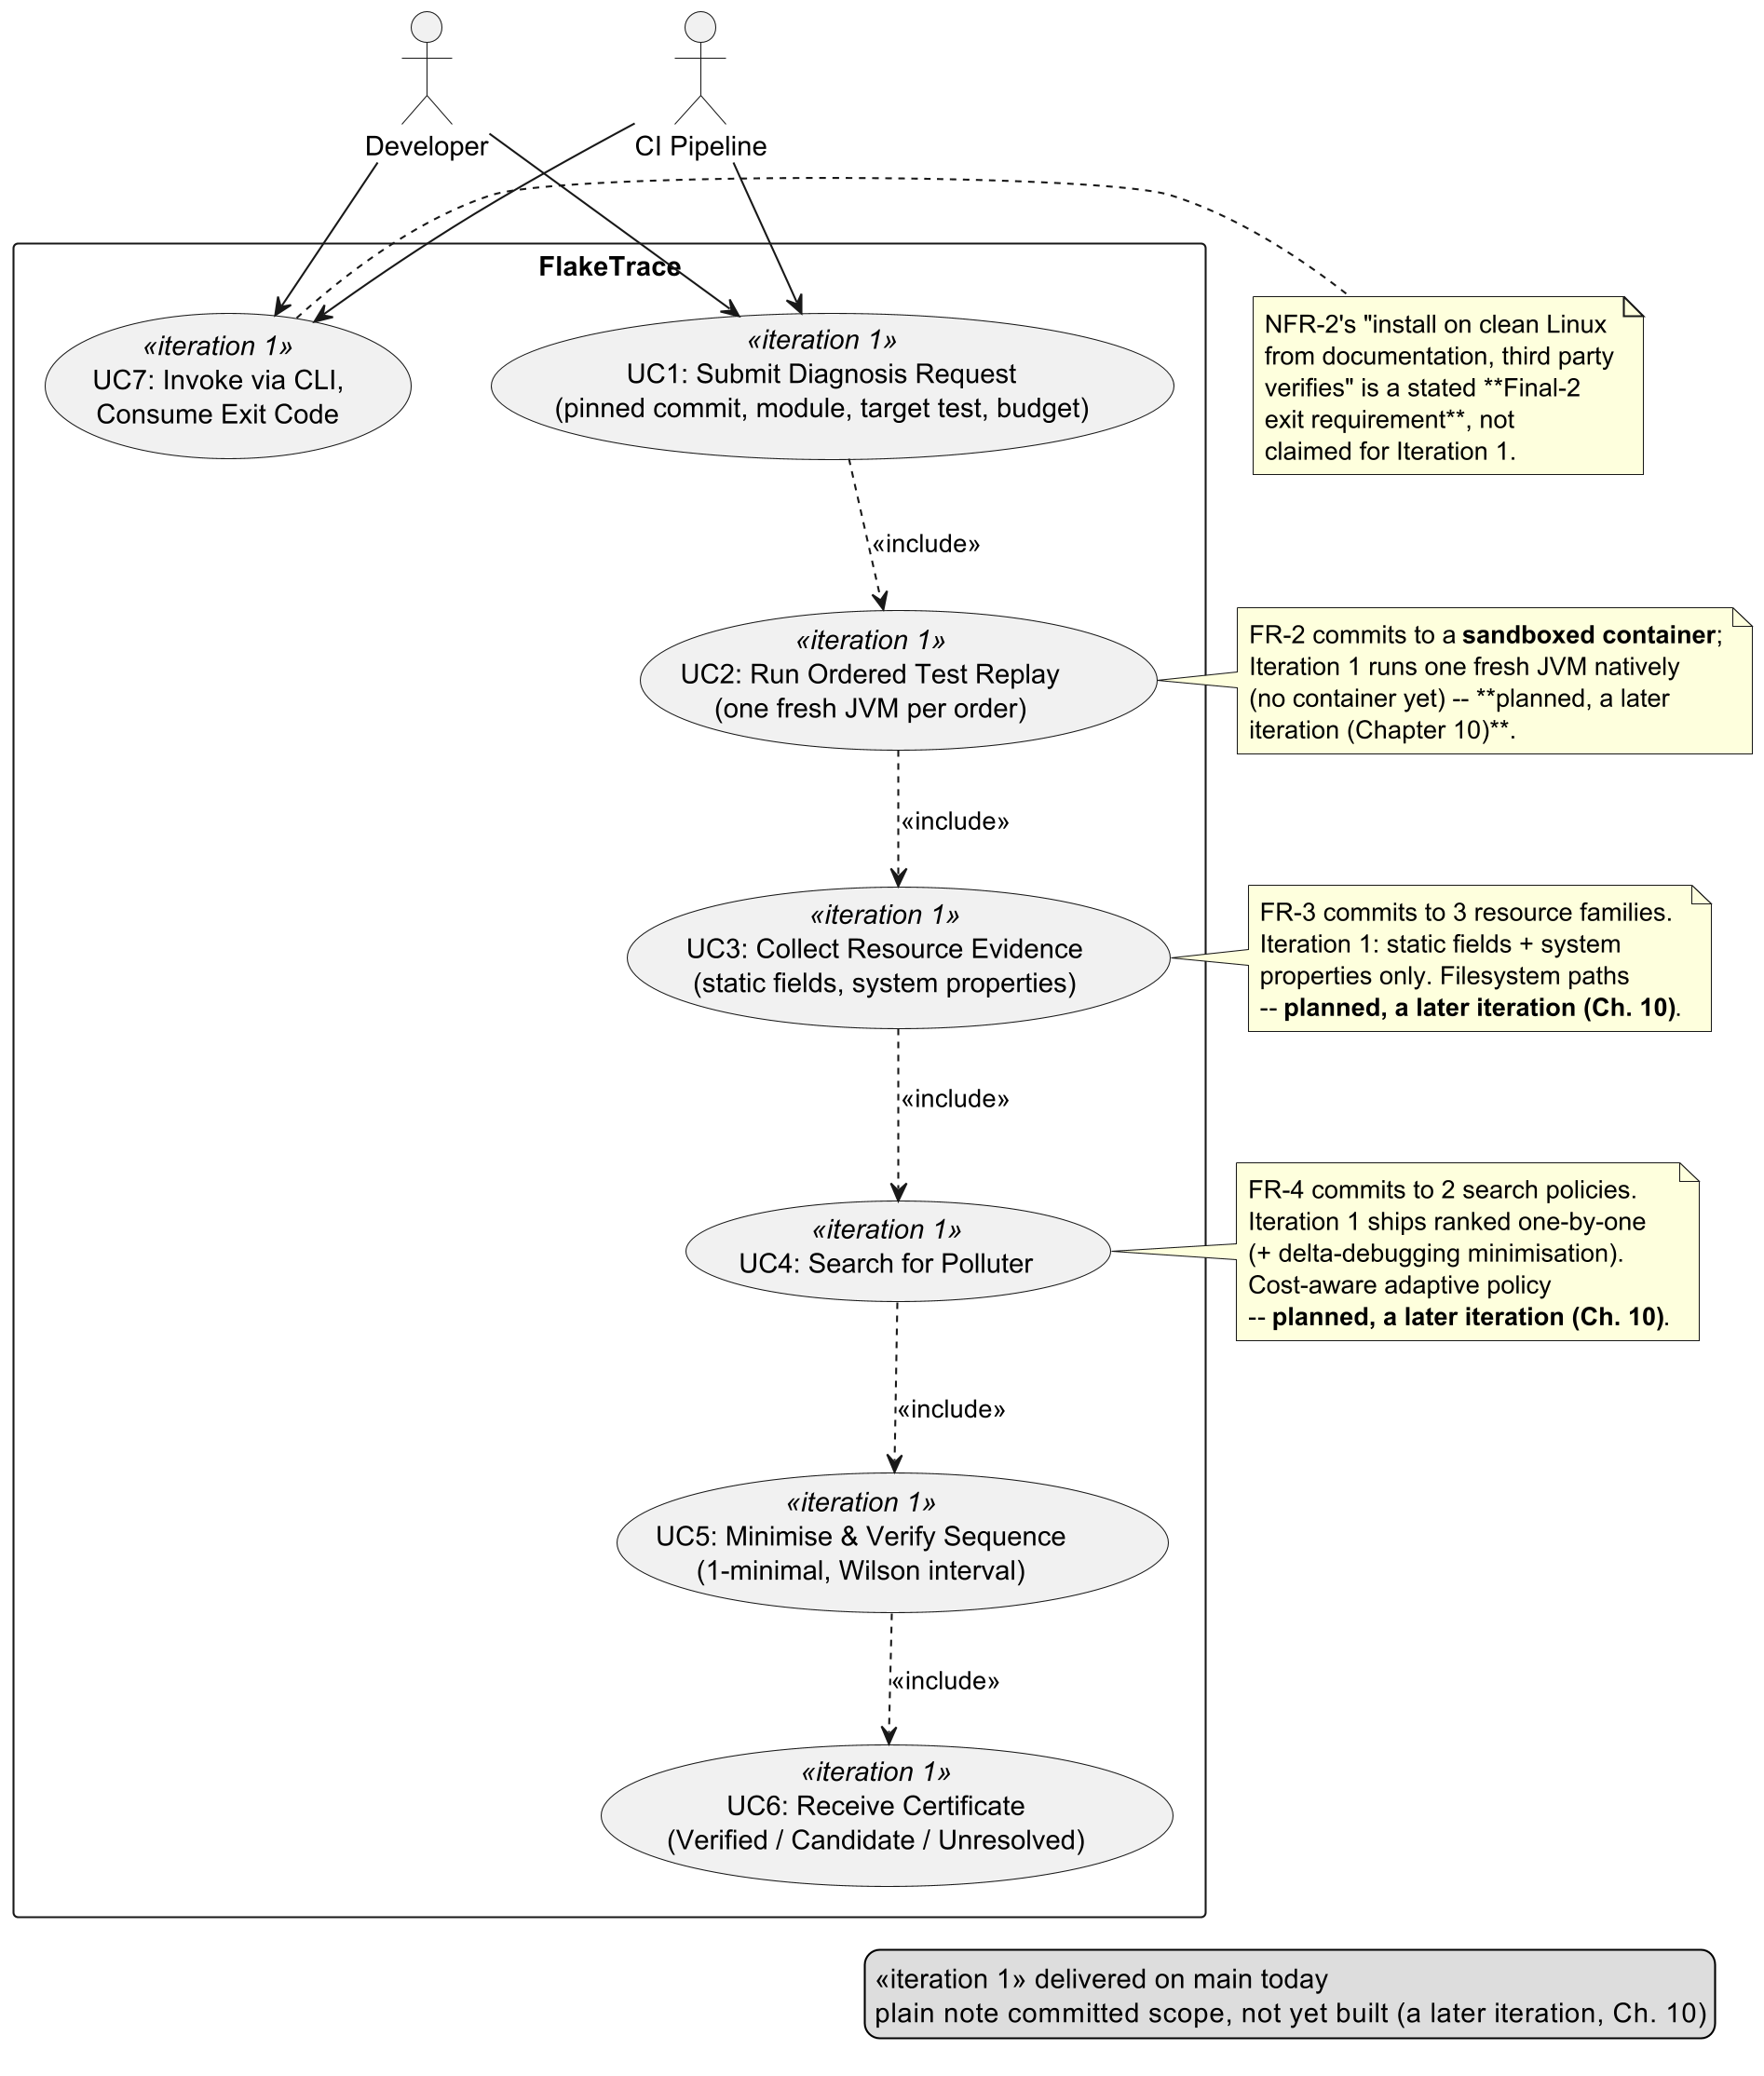
\includegraphics[width=0.85\textwidth]{figures/m3/use_cases}
  \caption{FlakeTrace use case diagram}\label{ch4:fig:usecases}
\end{figure}
Figure \ref{ch4:fig:usecases} shows the whole committed project, not only what Iteration 1
delivers: every use case carries the \texttt{<<iteration 1>>} stereotype because all seven are
implemented on \texttt{main} today, but the attached notes mark exactly which part of each
FR's full commitment is still FYP-2 work (container sandboxing, the filesystem resource
family, the cost-aware adaptive search policy, and NFR-2's clean-machine deployment check) ---
checked against the real code (\texttt{runner/}, \texttt{evidence/}) while drawing this
diagram, not assumed from the proposal.
\section{Detailed Use Cases}
\section{Functional Requirements}
\subsection{Module 1}
\subsection{Module 2}
\section{Non-Functional Requirements}\label{ch4:sec:nfr}
\subsection{Reliability}
\subsection{Usability}
\subsection{Performance}
\subsection{Security}
\section{Acceptance Criteria}
Define objective acceptance checks for important requirements.
\section{Requirements Traceability}
Trace important requirements to modules, design elements, implementation, and tests.

% ===========================================================================
% OWNER: M2 (Abdul Raffay) for 5.1-5.5; M1 for 5.6-5.8 (in chapter5_data_behaviour.tex)
% GRADED BY: Form 3 #5 Architecture & component/interface design (15) - gate: diagrams must match the code
% DRAW FROM: docs/03-Design/architecture.md, docs/contracts/interfaces.md, report-schema.md, resource-evidence.md, docs/03-Design/decisions/ADR-001..008, runner/, evidence/, eval/ READMEs
% NOTE: Design Evolution must show the proposal block diagram next to the current architecture and say what changed and which ADR changed it
% Rules: mid-eval-report/CLAUDE.md. Do not edit a file you do not own.
% ===========================================================================
\chapter{System Design}
\section{System Architecture}
% Current architecture (M2): diagrams/m2/architecture.puml -> figures/m2/architecture.png
\placeholderfig{ch5:fig:arch}{FlakeTrace architecture at Iteration 1 (as implemented)}{M2}
\section{Architectural Components}
\section{Interfaces and Dependencies}
\section{Architecture Decisions and Rationale}
\section{Design Evolution}
Show important design changes since the proposal and justify them.
\begin{figure}[H]\centering
  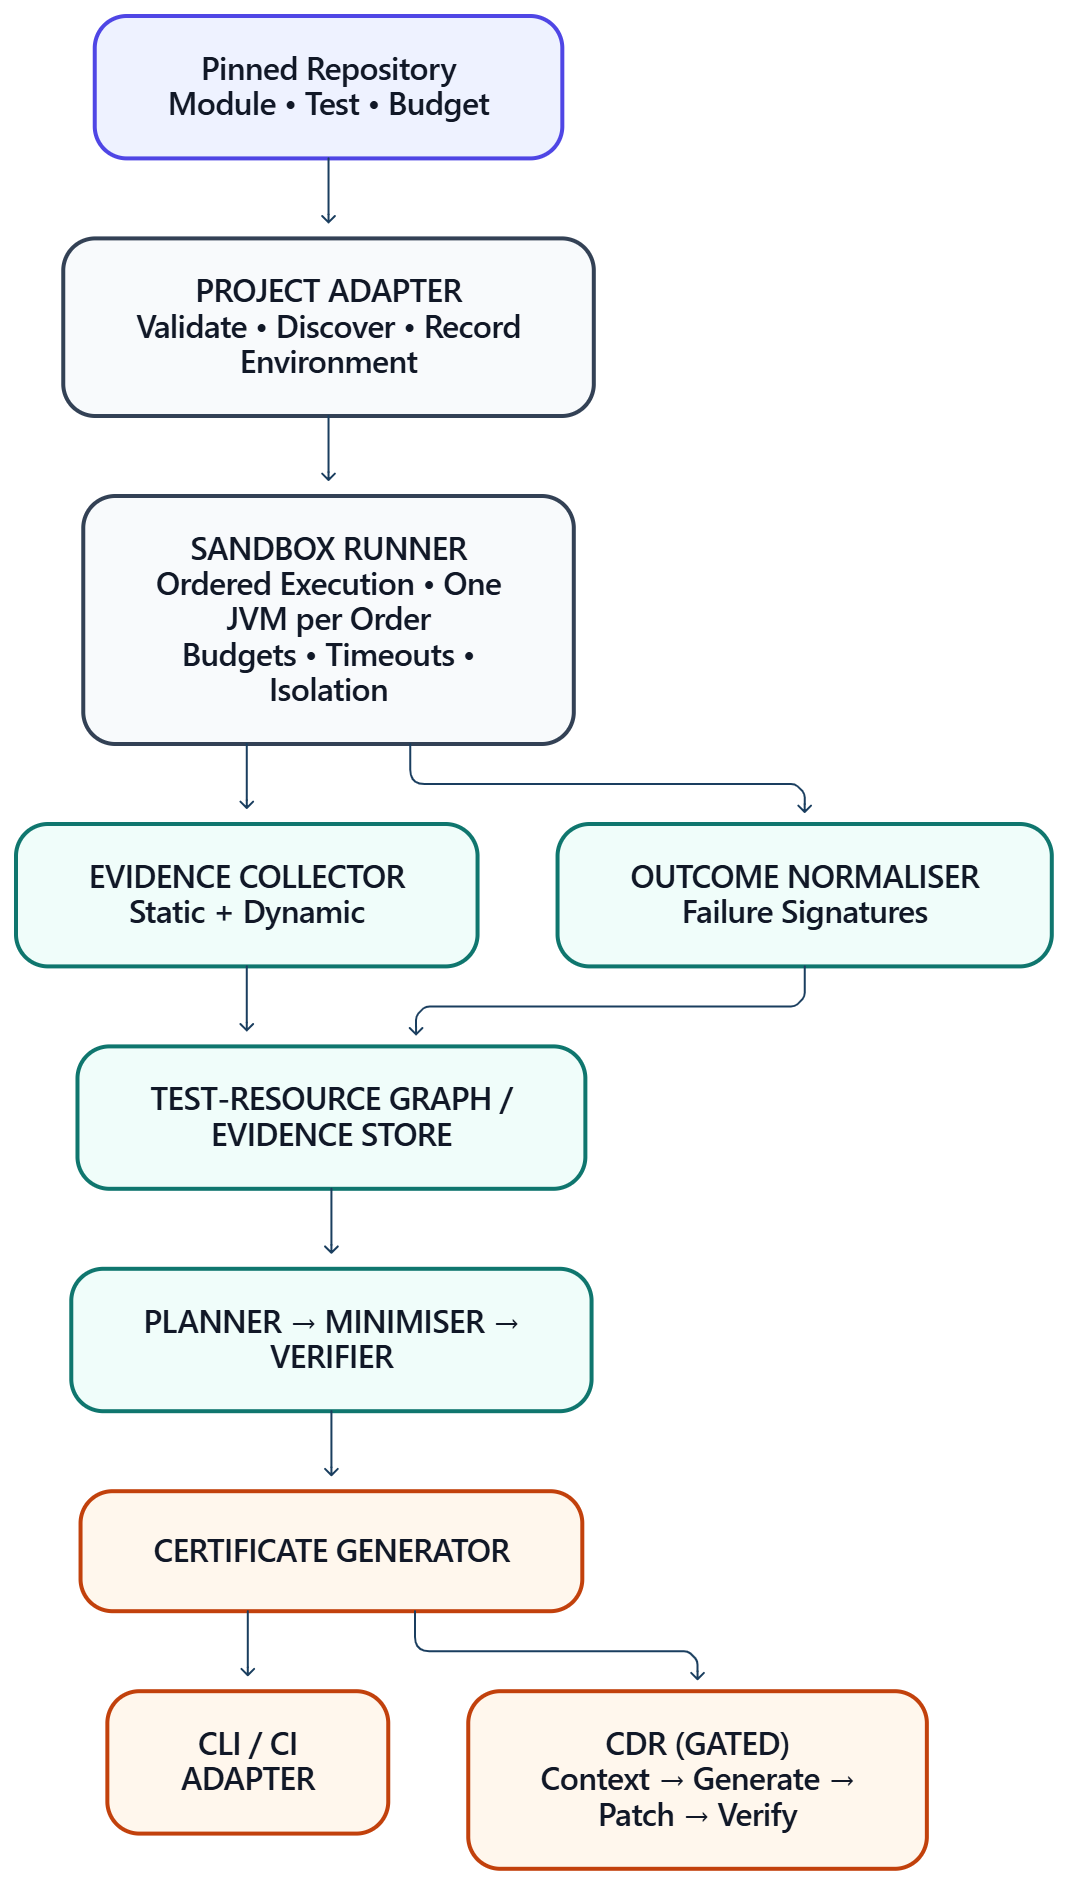
\includegraphics[width=0.85\textwidth]{figures/shared/proposal_block_diagram}
  \caption{System block diagram as presented at the proposal defence}\label{ch5:fig:proposal-arch}
\end{figure}
% Sections 5.6-5.8 are owned by M1:
% ===========================================================================
% OWNER: M1 (Zoya Ahmad); diagrams contributed by M2 and M3 as listed below
% GRADED BY: Form 3 #6 Data / process / behaviour design (10) - artefacts must be project-specific and explained in text
% DRAW FROM: eval/schema/report.schema.json, docs/contracts/*, evidence/extract.py, runner/diagnose.py, search.py, minimise.py, verify.py, eval/outcome.py
% NOTE: Each diagram is explained in prose: what it shows, and which code it was drawn from
% Rules: mid-eval-report/CLAUDE.md. Do not edit a file you do not own.
% ===========================================================================
% Included from chapter5_design.tex — no \chapter here.
\section{Domain Model}
\section{Data Design}
% Report data model (M1): diagrams/m1/report_data_model.puml -> figures/m1/report_data_model.png
\placeholderfig{ch5:fig:datamodel}{Diagnosis report data model (from report.schema.json)}{M1}
\section{Process / Behavior Design}
Include appropriate activity, sequence, state, DFD, ERD/schema, class, component, or other project-specific artefacts.
% Evidence extraction data flow (M1): diagrams/m1/evidence_dataflow.puml
\placeholderfig{ch5:fig:evidence-dfd}{Static evidence extraction: from bytecode to resource edges}{M1}
% Diagnose sequence (M2): diagrams/m2/diagnose_sequence.puml
\placeholderfig{ch5:fig:diagnose-seq}{Sequence of a \texttt{diagnose} run across the three components}{M2}
% Search pipeline activity (M2): diagrams/m2/search_activity.puml
\placeholderfig{ch5:fig:search-activity}{Reproduce, polluter search, minimisation and verification}{M2}
% Outcome decision (M3): diagrams/m3/outcome_decision.puml
\placeholderfig{ch5:fig:outcome}{Outcome decision: Verified, Candidate and typed Unresolved reasons}{M3}


% ===========================================================================
% OWNER: M2 (Abdul Raffay) for the frame; each member owns their module file
% GRADED BY: Form 3 #7 Implementation documentation (15) - gate: setup must be reproducible
% DRAW FROM: README.md (Run the checks), runner/README.md, evidence/README.md, eval/README.md, docs/04-Implementation/*, docs/08-MidEval/demo-plan.md, docs/evidence-m1/2/3.md
% NOTE: Setup commands must be copied from README.md and actually work; state what is mocked (demo-plan.md)
% Rules: mid-eval-report/CLAUDE.md. Do not edit a file you do not own.
% ===========================================================================
\chapter{Iteration 1: Design and Implementation}
\section{Iteration Objectives}
\section{Selected Use Cases / Features}
\section{Design}
\section{Implementation}
\section{Completed Features / Module}
\section{Technical Implementation Details}
Describe important files, classes, functions, algorithms, configurations, and technical decisions.
% ===========================================================================
% OWNER: M1 (Zoya Ahmad)
% GRADED BY: Form 3 #7
% DRAW FROM: evidence/README.md, evidence/extract.py, docs/04-Implementation/evidence-collector.md, docs/evidence-m1.md, ADR-002, ADR-006
% Rules: mid-eval-report/CLAUDE.md. Do not edit a file you do not own.
% ===========================================================================
\subsection{Resource Evidence Extraction (Member 1)}\label{ch6:sec:m1}
Member 1's module is the \path{evidence/} package. Given a polluter and a victim found by
Member 2's runner, it names the shared resource the polluter writes and the victim reads, and the
exact bytecode locations of that write and read. It works only from the project's compiled
classes, read with the JDK's \texttt{javap}: it runs no tests, adds no instrumentation and never
writes to the project (ADR-001, ADR-002). It is 716 lines of Python in one file, using only the
standard library, with 505 lines of tests (\texttt{wc -l}, 12 October 2026). Figure~\ref{ch5:fig:evidence-dfd}
shows its data flow.

\subsubsection{Files and main functions}
{\small
\begin{longtable}{>{\raggedright\arraybackslash}p{0.27\textwidth}>{\raggedright\arraybackslash}p{0.07\textwidth}>{\raggedright\arraybackslash}p{0.54\textwidth}}
\caption{Files of the resource evidence module}\label{ch6:tab:m1-files}\\
\toprule
File & Lines & Job\\
\midrule
\endfirsthead
\toprule
File & Lines & Job\\
\midrule
\endhead
\path{extract.py} & 716 & The extractor and its command line; main functions below\\
\path{tests/test_extract.py} & 505 & 39 \texttt{unittest} tests in seven classes, run on real
  \texttt{javap} output\\
\path{tests/resources/m1-selftest/} & -- & A small Maven project of ten Java files written as test
  input (lifecycle methods, call depth, JUnit~3, unsupported cases); not part of the fixture\\
\path{tools/measure_depth.py} & 70 & Measures accesses, unsupported observations, \texttt{javap}
  calls and time per depth; produced the depth data behind ADR-006\\
\path{javap-dumps/} & -- & Saved \texttt{javap} output quoted as evidence in
  \path{docs/evidence-m1.md}\\
\bottomrule
\end{longtable}}

The main functions in \path{extract.py}, in the order a pair is analysed:
\begin{itemize}
\item \texttt{Project.load}: runs \texttt{javap -v -p -c} on one class and parses it into
  \texttt{ClassInfo}, \texttt{Method} and \texttt{Instruction} objects, cached per class.
\item \texttt{find\_roots}: the test method plus its lifecycle methods (\texttt{@Before},
  \texttt{@After}, \texttt{@BeforeClass}, \texttt{@AfterClass}, JUnit~3 \texttt{setUp} and
  \texttt{tearDown}) and static initialisers, collected from the test class and its project
  superclasses; a method overridden in a subclass is skipped, because it never runs.
\item \texttt{walk\_root}, \texttt{scan\_method}, \texttt{scan\_call}, \texttt{follow\_call}: a
  breadth-first walk from each root that classifies each instruction and follows calls into
  project classes up to the depth limit.
\item \texttt{analyse\_test}: all accesses, unsupported observations and library calls not
  followed, for one test.
\item \texttt{find\_edges}: the resources the polluter writes and the victim reads.
\item \texttt{analyse\_pair}: both tests and their edges, deepening when needed.
\item \texttt{report\_fields}: turns a pair into the three report fields and the limitations.
\item \texttt{main}: the command line, \texttt{python3 -m evidence.extract}, which prints JSON and
  exits 0 (done), 1 (\texttt{javap} missing or failed) or 2 (input error).
\end{itemize}

\subsubsection{How extraction works}
For each root, \texttt{walk\_root} scans the method's bytecode one instruction at a time and queues
the project methods it calls, breadth-first, so every access is reported at the shortest call depth
at which it can be reached. Each method is scanned at most once per root, which also stops recursion
and call cycles. Listing~\ref{ch6:lst:m1-scan} shows the core of the scan.

\begin{lstlisting}[language=Python,basicstyle=\footnotesize\ttfamily,columns=fullflexible,keepspaces=true,caption={Core of \texttt{scan\_method}, abridged (\texttt{evidence/extract.py})},label=ch6:lst:m1-scan]
for index, ins in enumerate(method.instructions):
    owner = ins.owner or info.name
    if ins.opcode in ("getstatic", "putstatic"):
        declaring = project.declaring_class(owner, ins.name)
        resource = {"kind": "static-field",
                    "class": declaring, "field": ins.name}
        access = "READ" if ins.opcode == "getstatic" else "WRITE"
        result["accesses"].append(make_access(
            "static-field", resource, access, walk["via"],
            info, method, ins.offset, walk["path"]))
    elif ins.opcode == "invokedynamic":
        result["unsupported"].append(observation(
            "INVOKEDYNAMIC", info, method, ins, ...))
    elif ins.opcode.startswith("invoke"):
        scan_call(project, chain_names, info, method,
                  index, owner, walk, result)
\end{lstlisting}

Each instruction is classified as follows:
\begin{itemize}
\item \texttt{getstatic} and \texttt{putstatic} are a READ and a WRITE of a static field. The field is
  named by the class that \emph{declares} it, so a field reached through a subclass is still one
  resource.
\item A call to \texttt{System.getProperty}, \texttt{Integer.getInteger}, \texttt{Long.getLong} or
  \texttt{Boolean.getBoolean} is a READ of a system property. A call to
  \texttt{System.setProperty} or \texttt{clearProperty} is a WRITE, but only when every argument is pushed by one simple instruction
  right before the call and the first is a constant string (\texttt{constant\_key}); otherwise
  the call is reported as unsupported.
\item A call into a project class is followed one level deeper (\texttt{follow\_call}). A call into
  the JDK or a library is listed in \texttt{external\_calls\_not\_followed}.
\item Anything the extractor cannot model becomes a typed \emph{unsupported observation} with its
  location, never a guess: \texttt{REFLECTION}, \texttt{INVOKEDYNAMIC},
  \texttt{VIRTUAL\_\allowbreak DISPATCH} (only the named target is followed, not subclass overrides),
  \texttt{UNRESOLVED\_\allowbreak CALL}, \texttt{SYSPROP\_\allowbreak NON\_\allowbreak CONSTANT\_\allowbreak KEY},
  \texttt{SYSPROP\_\allowbreak BULK}, \texttt{IMPLICIT\_\allowbreak CLINIT} (a static initialiser
  that may run on first use), \texttt{DEPTH\_\allowbreak LIMIT} and
  \texttt{JUNIT\_\allowbreak RULE\_\allowbreak OR\_\allowbreak RUNNER}.
\end{itemize}
Every access records the resource, READ or WRITE, the class, method and bytecode offset, the root
it was reached from (\texttt{via}, for example \texttt{TEST\_METHOD} or \texttt{BEFORE}) and the call
path. \texttt{find\_edges} then keeps each resource the polluter writes and the victim reads, with
every write and read location. Writes made by the victim itself are not edges.

\subsubsection{Call depth and auto-deepening}\label{ch6:sec:m1-depth}
The depth is how many calls deep the walk follows from a root: depth~1 scans only the root's own
bytecode, depth~2 also the project methods it calls, and so on. Each extra level finds more but costs
more time and adds more code that is reachable but may never run. The team first fixed the default at
2 with a maximum of 3 (ADR-002). Measurements on the two real fastjson cases from the proof of concept
showed that this was not enough (Table~\ref{ch6:tab:m1-depth}): the victims reach the shared field
only inside constructors, four or five calls deep.

{\small
\begin{longtable}{>{\raggedright\arraybackslash}p{0.10\textwidth}>{\raggedright\arraybackslash}p{0.12\textwidth}>{\raggedright\arraybackslash}p{0.22\textwidth}>{\raggedright\arraybackslash}p{0.22\textwidth}>{\raggedright\arraybackslash}p{0.18\textwidth}}
\caption{Edges found per depth on fastjson (\texttt{docs/evidence-m1.md}, 10 October 2026)}\label{ch6:tab:m1-depth}\\
\toprule
Case & Depth & Real candidates with an edge & Other candidates with an edge & Seconds, all candidates\\
\midrule
\endfirsthead
\toprule
Case & Depth & Real candidates with an edge & Other candidates with an edge & Seconds, all candidates\\
\midrule
\endhead
FJ-01 & 1--3 & 0 of 42 & 0 of 30 & 22.4--30.2\\
FJ-01 & 4 & 42 of 42 & 1 of 30 & 34.8\\
FJ-01 & 5 & 42 of 42 & 1 of 30 & 45.8\\
FJ-02 & 1--3 & 0 of 24 & 0 of 698 & 143.3--156.1\\
FJ-02 & 4 & 1 of 24 & 0 of 698 & 163.2\\
FJ-02 & 5 & 24 of 24 & 0 of 698 & 180.7\\
\bottomrule
\end{longtable}}

A ``real'' candidate is one that changed the victim's result when the proof of concept ran it first.
Raising the fixed depth to~5 would make every pair pay the deepest cost: one pair took 3--6~s at
depth~2, but 7.5~s for FJ-01 at depth~4 and 26.3~s for FJ-02 at depth~5 (ADR-006). The team therefore
adopted \emph{auto-deepening} (ADR-006), implemented in \texttt{analyse\_pair}:
\begin{enumerate}
\item analyse both tests at the requested depth (default~2);
\item if there is no edge \emph{and} a walk stopped at the depth limit (\texttt{DEPTH\_LIMIT}),
  repeat one level deeper;
\item stop at the first depth with an edge, when nothing was cut off, or at depth~5.
\end{enumerate}
The pair records \texttt{depth\_requested} and \texttt{depth\_used}, and when the reported evidence
is deeper than the default, \texttt{report\_fields} adds a limitation saying that deeper evidence is
more likely to be code that never runs. On the fixture, every ground-truth edge is found at depth~2
without deepening.

\subsubsection{How the runner uses the module}
Member 2's \texttt{diagnose} command calls the module once the polluters are known
(\texttt{resource\_fields} in \path{runner/cli.py}): it runs \texttt{analyse\_pair} once for each
polluter with the victim, and \texttt{combine\_fields} joins the results. With one polluter the
report holds \texttt{report\_fields} unchanged. With several, it shows the first polluter's edge and
names the others in \texttt{limitations}, but only if \emph{every} polluter has an edge; otherwise the
three resource fields are \texttt{null}, so that a \texttt{VERIFIED} result always means every
blamed test has a found mechanism. The report holds one resource and one location per side, so
\texttt{report\_fields} shows the first edge and its first write and read, and lists any other edges
and locations in \texttt{limitations}. The module can also be run on its own, for example on F2:
\begin{lstlisting}[basicstyle=\footnotesize\ttfamily,columns=fullflexible,keepspaces=true,breaklines=true]
python3 -m evidence.extract --classes fixtures/od-fixture/target/classes \
    --test-classes fixtures/od-fixture/target/test-classes \
    --polluter odfixture.FeaturePolluterTest#enableTurbo \
    --victim odfixture.FeatureVictimTest#expectsTurboDisabled
\end{lstlisting}
Run on 12 October 2026 (main \texttt{82df9fa}), it exited 0 and its \texttt{pair} section reported
one edge, \texttt{sysprop:odfixture.turbo}: written at \texttt{FeaturePolluterTest.enableTurbo}
offset~4 and read at \texttt{FeatureFlags.isTurboEnabled} offset~2, a method the victim calls, so
the read is at depth~2 (\texttt{depth\_used}~2).

\subsubsection{Setup and running}
The module needs Python~3 and a JDK~8 or newer with \texttt{javap} on the path (or
\texttt{FLAKETRACE\_JAVAP} set to another \texttt{javap}); it has no other dependencies. Its tests
need the fixture and the self-test project compiled first. From the repository root:
\begin{lstlisting}[basicstyle=\footnotesize\ttfamily,columns=fullflexible,keepspaces=true,breaklines=true]
mvn -B -q -f fixtures/od-fixture/pom.xml test-compile
mvn -B -q -f evidence/tests/resources/m1-selftest/pom.xml test-compile
FLAKETRACE_REQUIRE_JVM=1 python3 -m unittest -v evidence.tests.test_extract
\end{lstlisting}
\texttt{FLAKETRACE\_REQUIRE\_JVM=1} turns a missing \texttt{javap} into a failure instead of skipped
tests. On Windows Command Prompt the variable is set with \texttt{set FLAKETRACE\_REQUIRE\_JVM=1} and
Python is started with \texttt{py}. These are the same commands as the \texttt{evidence} job in
\path{.github/workflows/ci.yml}, which runs them on Ubuntu with JDK~8 for every pull request.

On 12 October 2026, on main \texttt{82df9fa}, both builds exited 0 and the suite reported
\texttt{Ran 39 tests in 60.392s \ldots{} OK}. This run was made with Claude in the team's cloud
environment (Linux, Maven 3.9.11, OpenJDK and \texttt{javap} 21.0.12.1, Python 3.13.16), not on a
member's own machine; it is recorded in \path{docs/evidence-m1.md}.

\subsubsection{Results}
All results are recorded in \path{docs/evidence-m1.md}.
\begin{itemize}
\item \textbf{Fixture against its ground truth.} Every fixture test is tried as polluter against
  every other as victim: 240 ordered pairs over 16 tests. Edges appear for exactly the ground-truth
  pairs, each on the ground-truth resource, at the default depth without deepening: F1
  (\texttt{Config.mode}), F2 (\texttt{odfixture.turbo}, read at depth~2), F3 (\texttt{Toggles.flagA}
  and \texttt{flagB}, one per polluter) and F4 (\texttt{LateFlag.isSet}). No test gets an edge to N1,
  N2 or N3. The ground truth was written by Member~3 before any run.
\item \textbf{End to end.} The same edges appear in the reports of Table~\ref{ch8:tab:fixture-results},
  where all four order-dependent cases are \texttt{VERIFIED}.
\item \textbf{A real project.} On fastjson at the proof of concept's pinned commit, built unmodified,
  the edges for FJ-01 and FJ-02 appear at depths~4 and~5 (Table~\ref{ch6:tab:m1-depth}), on the
  fields \texttt{JSON.defaultTimeZone} and \texttt{JSON.defaultLocale}; the offsets on FJ-01's read path were checked
  against the saved \texttt{javap} output (\path{evidence/javap-dumps/phase5-fastjson.txt}). Both cases are brittle tests whose earlier test is a state-setter,
  which the module treats the same way: one test writes, the other reads.
\end{itemize}

\subsubsection{Testing}
The 39 tests in \path{evidence/tests/test_extract.py} run the real extractor on real
\texttt{javap} output; nothing is mocked. They are grouped in seven classes:
\texttt{DepthOneExtractionTest} (the exact accesses and offsets, JUnit~3 and~4 lifecycle
attribution, unsupported cases reported, not guessed), \texttt{CallDepthTest} (what each depth adds,
the depth limit, recursion), \texttt{PairSelfTest} (edge rules, including writes in \texttt{setUp} and
static initialisers), \texttt{DeepeningTest}, \texttt{FixturePairTest} (F1--F3 and the report-field
shape), \texttt{GroundTruthTest} (the 240-pair check above) and \texttt{CommandLineTest} (output and
exit codes). When the ground-truth check was added, it was itself checked: forcing depth~1 made it
fail on the missing F2 pair, and altering the ground truth in memory made it fail as well.

\subsubsection{Limitations and a failure case}
Every report carries the module's seven fixed limitations (Section~\ref{ch1:sec:constraints}). Three
matter most in practice:
\begin{itemize}
\item \textbf{A false edge.} On FJ-01 at depths~4 and~5, one of the 30 candidates that did not affect
  the victim still gets an edge: \texttt{DateTest2\#test\_date} writes \texttt{JSON.defaultTimeZone},
  but sets it and restores the old value in \texttt{tearDown}. The extractor sees a WRITE because it
  does not model the values written. This is why an edge alone never makes a result
  \texttt{VERIFIED}: the polluter must also be confirmed by reruns.
\item \textbf{Two edges, one cause.} On both fastjson cases the state-setter's \texttt{setUp} writes
  both \texttt{defaultTimeZone} and \texttt{defaultLocale}, and the victim reads both, so both are
  edges. Static analysis cannot say which one causes the failure; from the test's own constants it
  is the time zone, but that has not been confirmed by a run. The report shows the first edge and
  names the other in \texttt{limitations}.
\item \textbf{Evidence from one real project.} Two real cases from fastjson, a library built around
  global static configuration, are favourable to this kind of analysis. Whether depth~5 is enough
  elsewhere is not yet known; where static analysis finds nothing, the result is
  \texttt{UNRESOLVED} with \texttt{NO\_SUPPORTED\_RESOURCE\_EVIDENCE}, never ``independent'', and
  runtime evidence is the planned fallback (ADR-001).
\end{itemize}

% ===========================================================================
% OWNER: M2 (Abdul Raffay)
% GRADED BY: Form 3 #7
% DRAW FROM: runner/README.md, runner/*.py, runner/harness/FtHarness.java, docs/04-Implementation/{sandbox-runner,diagnosis-runs,diagnose-cli}.md, docs/evidence-m2.md, ADR-003/004/005/007/008
% Rules: mid-eval-report/CLAUDE.md. Do not edit a file you do not own.
% ===========================================================================
\subsection{Ordered Runner, Polluter Search, Minimisation and CLI (Member 2)}\label{ch6:sec:m2}
Member 2's module is the \path{runner/} package: it runs tests in a chosen order, finds the polluter, shrinks the failing order, repeats it, and is the command that joins the three packages. It is 1{,}119 lines of Python and Java, with 1{,}488 lines of tests (\texttt{wc -l}, 11 October 2026).

\subsubsection{Files and main functions}
{\small
\begin{longtable}{>{\raggedright\arraybackslash}p{0.26\textwidth}>{\raggedright\arraybackslash}p{0.07\textwidth}>{\raggedright\arraybackslash}p{0.55\textwidth}}
\caption{Files of the runner module}\label{ch6:tab:m2-files}\\
\toprule
File & Lines & Job\\
\midrule
\endfirsthead
\toprule
File & Lines & Job\\
\midrule
\endhead
\path{order_runner.py} & 220 & \texttt{OrderRunner.run\_ordered}: one fresh JVM per order; \texttt{maven\_test\_classpath}; failure-signature normalisation\\
\path{harness/FtHarness.java} & 122 & Runs the listed tests in order with \texttt{JUnitCore}; lists test methods for discovery\\
\path{discovery.py} & 31 & \texttt{discover\_order}: test classes by Surefire's default include patterns, methods from JUnit\\
\path{search.py} & 55 & \texttt{reproduce} (first real failure becomes the reference); \texttt{find\_polluter} (one-by-one)\\
\path{orders.py} & 69 & \texttt{distinct\_shuffles}, \texttt{search\_orders}: class-first shuffled orders (ADR-008)\\
\path{minimise.py} & 55 & \texttt{ddmin}: 1-minimal polluter set (ADR-007)\\
\path{verify.py} & 33 & \texttt{repeat}: $n$ runs, matching and any-signature failure counts\\
\path{integrity.py} & 40 & \texttt{snapshot}, \texttt{compare}: SHA-256 of the project's files before and after\\
\path{recording.py} & 54 & \texttt{RecordingRunner}: writes every JVM run to the execution record\\
\path{diagnose.py} & 208 & \texttt{diagnose}, \texttt{run\_steps}: the whole diagnosis, returns raw counts\\
\path{cli.py}, \path{__main__.py} & 232 & \texttt{py -m runner diagnose}: options, evidence per polluter, report, summary, exit codes\\
\bottomrule
\end{longtable}}

\subsubsection{Ordered runner}
\texttt{OrderRunner} compiles \path{FtHarness.java} once with \texttt{javac -source 8 -target 8}. Each call to \texttt{run\_ordered(order)} then starts \texttt{java FtHarness <result-file>} in the analysed project's folder, with the project's own test classpath, sends the test list on standard input, and waits at most 120\,s. The harness runs each test with JUnit's \texttt{JUnitCore.run(Request.method(...))} and writes one line per test to the result file, so output printed by a test cannot corrupt the results. Python then turns each failure into a \texttt{FailureSignature}:
\begin{itemize}
  \item \textbf{exception type:} the class of the thrown exception (not its cause);
  \item \textbf{stack trace:} the frames from the throw point down to the first frame of JUnit's runner, Java reflection or the harness. Those lower frames differ between JDK 8 and JDK 21 and say nothing about the failure;
  \item \textbf{message:} the first line with numbers, hexadecimal ids, timestamps and paths masked. It is stored but not compared, because the same bug can print different values on each run.
\end{itemize}
The contract requires every test in the order to appear in the result, so the runner never drops one (Table~\ref{ch6:tab:m2-always}).

{\small
\begin{longtable}{>{\raggedright\arraybackslash}p{0.42\textwidth}>{\raggedright\arraybackslash}p{0.46\textwidth}}
\caption{How the runner reports every test (\texttt{runner/README.md})}\label{ch6:tab:m2-always}\\
\toprule
Situation & Reported as\\
\midrule
\endfirsthead
\toprule
Situation & Reported as\\
\midrule
\endhead
JVM runs longer than 120\,s & failure, \texttt{flaketrace.Timeout}\\
JVM exits before reporting a test (crash, \texttt{System.exit}) & failure, \texttt{flaketrace.JvmCrash}, exit code in the message\\
Class or method not found & failure with JUnit's own exception\\
\texttt{@Ignore} or a failed \texttt{Assume} & failure, \texttt{flaketrace.NotExecuted}: a skip never counts as a pass\\
The same test twice in one order & \texttt{ValueError} before any JVM starts\\
\bottomrule
\end{longtable}}

The \texttt{flaketrace.*} types mark failures the tool produced, not the test. Such a failure is counted as ``failed for any reason'' but never becomes the reference signature and never counts as a reproduction.

\subsubsection{Diagnosis flow}
\texttt{diagnose()} hashes the project, builds the classpath, discovers the tests, wraps the runner in a \texttt{RecordingRunner}, and calls \texttt{run\_steps} (Figure~\ref{ch5:fig:search-activity}). It returns a \texttt{DiagnosisRuns} object with raw counts and one of four statuses (Table~\ref{ch6:tab:m2-status}); it never decides the outcome, which is Member 3's \texttt{decide()}.

{\small
\begin{longtable}{>{\raggedright\arraybackslash}p{0.25\textwidth}>{\raggedright\arraybackslash}p{0.40\textwidth}>{\raggedright\arraybackslash}p{0.23\textwidth}}
\caption{Statuses returned by \texttt{diagnose()}}\label{ch6:tab:m2-status}\\
\toprule
Status & Meaning & Sequence repeated $n$ times\\
\midrule
\endfirsthead
\toprule
Status & Meaning & Sequence repeated $n$ times\\
\midrule
\endhead
\texttt{POLLUTER\_FOUND} & One earlier test, or a 1-minimal set found by \texttt{ddmin}, makes the victim fail with the reference signature & polluters + victim\\
\texttt{VICTIM\_FAILS\_ALONE} & The victim fails with nothing before it; no test is blamed & victim alone\\
\texttt{NO\_SINGLE\_POLLUTER} & A failure was seen but did not come back; no test is blamed & the failing order\\
\texttt{NOT\_REPRODUCED} & No real failure in $n$ runs of the order, in the shuffled orders, or in $n$ runs alone & the starting order\\
\bottomrule
\end{longtable}}

\subsubsection{Minimisation with ddmin}\label{ch6:sec:ddmin}
When no single earlier test makes the victim fail, \texttt{run\_steps} first runs the full order once more. Only if it fails again with the reference signature does \texttt{ddmin} (\path{runner/minimise.py}) shrink the tests before the victim; otherwise a one-off flaky failure would make every earlier test look guilty. Listing~\ref{ch6:lst:ddmin} is the core loop.

\begin{lstlisting}[language=Python,basicstyle=\footnotesize\ttfamily,columns=fullflexible,keepspaces=true,caption={Core of \texttt{ddmin} (\texttt{runner/minimise.py})},label=ch6:lst:ddmin]
current, k = list(prefix), 2
while len(current) > 1:
    chunks = _split(current, k)
    smaller = next((chunk for chunk in chunks if fails(chunk)), None)
    if smaller is not None:
        current, k = smaller, 2
        continue
    complements = ([t for t in current if t not in chunk] for chunk in chunks)
    smaller = next((rest for rest in complements if fails(rest)), None)
    if smaller is not None:
        current, k = smaller, max(k - 1, 2)
        continue
    if k >= len(current):
        break
    k = min(2 * k, len(current))
return current, runs
\end{lstlisting}

\texttt{fails(subset)} runs \texttt{subset + [victim]} in its original relative order in one fresh JVM and returns true only if the victim fails with the \emph{reference} signature; a crash or a different exception never removes a test. A cache keyed by the set of tests means no subset runs twice. The loop ends when \texttt{k} equals the set size, so its last round has tried removing each remaining test on its own: the result is \emph{1-minimal} (removing any one test makes the failure disappear), not necessarily the smallest set that exists.

On fixture F3 (run on 11 October 2026, Windows 11, JDK 21.0.9), the command printed \texttt{minimised: 14 earlier tests -> 2 polluters in 10 runs}, and the two polluters were the ground truth's \texttt{setFlagA} and \texttt{setFlagB}. The execution record of that run shows 65 JVM runs in total: 1 to reproduce, 20 alone, 14 for the one-by-one search, 10 for minimisation (including the one re-run of the full order) and 20 to verify.

\subsubsection{Verification and order search}
\texttt{repeat} (\path{runner/verify.py}) runs the final sequence $n$ times, each in a fresh JVM, and returns two counts: runs where the victim failed with the reference signature, and runs where it failed for any reason. The default is $n = 20$, agreed by all three members: 20 matching failures out of 20 give a Wilson lower bound of 0.839 and 19 out of 20 give 0.764, both above the 0.70 that Member 3's \texttt{decide()} requires for \texttt{VERIFIED} (\path{docs/contracts/interfaces.md}, question I3; ADR-004). The victim-alone check uses the same function on \texttt{[victim]}.

When the starting order never fails for real, \path{runner/orders.py} tries up to 31 distinct shuffled orders, one run each (ADR-008). Classes are shuffled first and then the methods inside each class, because JUnit never interleaves the methods of two classes; every seed is written to the execution record, so any shuffle can be replayed. In the worst case a diagnosis that never reproduces costs $20 + 31 + 20 = 71$ JVM runs. On the fixture, F4's discovered order never fails, and the failure was reproduced in the second shuffled order (seed 1); N3 never failed in 20 runs of its order, 31 shuffled orders or 20 runs alone, and its report gives the bound ``failure rate below 0.161 (95\% Wilson), not proof of reliability'' (\path{docs/evidence-m2.md}, 11 October 2026).

\subsubsection{Command line}
\texttt{py -m runner diagnose} (\path{runner/cli.py}, ADR-005) takes the options in Table~\ref{ch6:tab:m2-options} and maps every result to an exit code (Table~\ref{ch6:tab:m2-exit}). A known error prints one line, \texttt{error: ...}, with no stack trace; an unexpected bug still prints its trace, on purpose.

{\small
\begin{longtable}{>{\raggedright\arraybackslash}p{0.15\textwidth}>{\raggedright\arraybackslash}p{0.17\textwidth}>{\raggedright\arraybackslash}p{0.56\textwidth}}
\caption{Options of \texttt{py -m runner diagnose}}\label{ch6:tab:m2-options}\\
\toprule
Option & Default & Meaning\\
\midrule
\endfirsthead
\toprule
Option & Default & Meaning\\
\midrule
\endhead
\texttt{-{}-project} & required & Maven project folder, must contain \texttt{pom.xml}\\
\texttt{-{}-victim} & required & failing test as \texttt{Class\#method}\\
\texttt{-{}-n} & 20 & repeat count\\
\texttt{-{}-records} & \texttt{flaketrace-\allowbreak records} & folder for the record and report; refused if inside the project\\
\texttt{-{}-order} & none & file with the real failing order, one \texttt{Class\#method} per line\\
\texttt{-{}-shuffles} & 31 & shuffled orders to try if the order never fails; 0 turns it off\\
\texttt{-{}-seed} & 0 & first shuffle seed\\
\bottomrule
\end{longtable}}

{\small
\begin{longtable}{>{\raggedright\arraybackslash}p{0.06\textwidth}>{\raggedright\arraybackslash}p{0.82\textwidth}}
\caption{Exit codes of \texttt{py -m runner diagnose}}\label{ch6:tab:m2-exit}\\
\toprule
Code & Meaning\\
\midrule
\endfirsthead
\toprule
Code & Meaning\\
\midrule
\endhead
0 & Report written, whatever the outcome, including \texttt{UNRESOLVED}\\
2 & Input is wrong: victim not \texttt{Class\#method}, no \texttt{pom.xml}, $n < 1$, records folder inside the project, bad \texttt{-{}-order} file, victim not among the project's tests\\
1 & A tool failed: Maven, \texttt{java}, \texttt{javac}, a timeout during discovery, or the extractor\\
3 & The diagnosis ran but no report can be built: \texttt{NO\_SINGLE\_POLLUTER}\\
\bottomrule
\end{longtable}}

Listing~\ref{ch6:lst:m2-f1} is the summary printed for fixture F1 on 11 October 2026 (the two lines with the report and record paths are left out).
\begin{lstlisting}[basicstyle=\footnotesize\ttfamily,columns=fullflexible,keepspaces=true,breaklines=true,breakatwhitespace=true,caption={Summary for F1 (exit code 0)},label=ch6:lst:m2-f1]
VERIFIED  odfixture.ConfigVictimTest#expectsDefaultMode
  polluter:   odfixture.ConfigPolluterTest#pollute
  resource:   static-field odfixture.Config mode (write odfixture.ConfigPolluterTest#pollute@1 -> read odfixture.ConfigVictimTest#expectsDefaultMode@1)
  reproduced: 20/20 (lower bound 0.839)   alone: 0/20
\end{lstlisting}

\subsubsection{Testing}
The module has 144 tests in nine files under \path{runner/tests/}. Most of the logic (search, minimisation, order search, recording) is tested against Member 3's \texttt{FakeOrderRunner}, which returns scripted outcomes without a JVM and exists only under \path{eval/tests/}; the order runner, \texttt{diagnose()} and the command are also tested with real JVM runs on the fixture. Without \texttt{java} or Maven the real tests are skipped, except in CI, where \texttt{FLAKETRACE\_REQUIRE\_JVM} turns a skip into a failure. All 144 passed in CI on Linux with JDK 8 in 105.2\,s (pull request \#49) and locally on Windows with JDK 21 in 344.8\,s (Table~\ref{ch6:tab:setup-results}).

Most tests were written before the code they check and were seen failing first; key tests were also checked by breaking the code on purpose and watching them fail (\path{docs/evidence-m2.md} records both for each task). Two examples: changing the alone check from \texttt{alone\_successes >= 1} to \texttt{>= 100} made \texttt{test\_victim\_failing\_alone\_stops\_before\_the\_search} fail; and a test that reads a 20{,}001-line \texttt{-{}-order} file within 5\,s failed at 33.4\,s, which exposed a quadratic duplicate check, after which the same file took 0.094\,s.

\subsubsection{Limitations and a failure case}
\begin{itemize}
  \item \textbf{No sandbox.} The analysed project's tests run as ordinary processes with the user's permissions; there is no container yet. FlakeTrace should only be run on projects the user trusts.
  \item \textbf{JUnit 3 and 4 only.} JUnit 5 is not supported. Each method is its own JUnit request, so \texttt{@BeforeClass} and \texttt{@AfterClass} run once per method, not once per class as under Maven Surefire.
  \item \textbf{Signatures within one JDK.} Frames from the JDK itself above the cut keep their line numbers, which differ between JDK versions, so such signatures are only compared within one diagnosis. Only the top-level exception is compared, not its cause.
  \item \textbf{Discovery order.} Tests are discovered in alphabetical order; Surefire's default runs them in file-system order. For a failure seen in CI, the real order should be passed with \texttt{-{}-order}.
  \item \textbf{No report for \texttt{NO\_SINGLE\_POLLUTER}.} The report schema has no reason for it, so the command exits with code 3 and only the execution record remains.
  \item \textbf{31 shuffles is an assumption.} The figure comes from a study of Python projects~\cite{gruber2021flaky}.
\end{itemize}

\textbf{Failure case: N2 on one laptop.} N2 is meant to fail at random. On 9 October 2026 its real-JVM test failed: \texttt{diagnose()} returned \texttt{NOT\_REPRODUCED}, because N2 failed in none of 40 runs of its order and none of 40 runs alone, although a design experiment earlier that day had seen it fail 18 times in 60 runs alone. A probe showed that \texttt{System.nanoTime()} on that laptop only returned multiples of 100, so N2's random condition could never come true there; why the earlier run differed was not found. The diagnosis was right and the test's assumption was wrong: the test now checks that no polluter is ever blamed and accepts \texttt{NOT\_REPRODUCED} when N2 never fails (\path{docs/evidence-m2.md}, ADR-004).

% ===========================================================================
% OWNER: M3 (Zarpash Nasim)
% GRADED BY: Form 3 #7
% DRAW FROM: eval/README.md, eval/*.py, eval/schema/, fixtures/od-fixture/, docs/05-Testing/fixture-suite.md, docs/evidence-m3.md
% Rules: mid-eval-report/CLAUDE.md. Do not edit a file you do not own.
% ===========================================================================
\subsection{Evaluation, Statistics and Report Assembly (Member 3)}
\todo{M3: files, Wilson interval, outcome decision, report schema, fixtures, limitations, real results from evidence-m3.md}

\section{Algorithms and Technical Decisions}
\section{Tools, Frameworks and Technologies}
\section{Demonstration Evidence}
\section{Iteration Outcome}

% ===========================================================================
% OWNER: M3 (Zarpash Nasim); M2 adds runner test rows by PR
% GRADED BY: Form 3 #8 Testing plan & tool/risk disclosure (15)
% DRAW FROM: docs/05-Testing/evaluation-plan.md, fixture-suite.md, .github/workflows/ci.yml, eval/tests, runner/tests, evidence/tests, eval/reports/*.json, docs/evidence-m1/2/3.md
% NOTE: Result tables come from tables/generated/ (scripts/json_to_tex.py), never typed by hand
% Rules: mid-eval-report/CLAUDE.md. Do not edit a file you do not own.
% ===========================================================================
\chapter{Testing and Early Validation}

\section{Testing Strategy}
The evaluation plan (\texttt{docs/05-Testing/evaluation-plan.md}) treats testing, evaluation and
acceptance as three different questions, and this chapter only answers the first:
\textbf{testing} asks whether the implementation meets its own requirements (unit, integration
and system checks); \textbf{evaluation} asks whether the approach is better under stated budgets
(baseline comparisons, ablations); \textbf{acceptance} asks whether the intended users would
actually use it (named-participant tasks). Evaluation is partly covered in Chapter 4's
Acceptance Criteria (Table \ref{ch4:tab:acceptance}) via claim B11's baseline work; full
acceptance testing is genuinely not started (Section \ref{ch8:sec:acceptance}).

Strategy, concretely: every component is unit-tested in isolation with real, scriptable fakes
confined to \texttt{*/tests/} (never imported by production code --- CLAUDE.md \S4); the fixture
project (\texttt{fixtures/od-fixture}) then exercises the whole pipeline end to end against
seven cases with pre-registered, before-any-run ground truth
(\texttt{fixtures/od-fixture/ground\_truth.json}); and every one of those checks runs in CI on
every push and pull request, not only locally.

\section{Test Levels and Techniques}\label{ch8:sec:levels}
Table \ref{ch8:tab:ci} lists the five real CI jobs (\texttt{.github/workflows/ci.yml}), each
testing a different level, all green on the current \texttt{main} tip.

\begin{table}[H]\centering
\caption{CI jobs and what they test}\label{ch8:tab:ci}
\begin{tabular}{p{2.6cm}p{4.0cm}p{6.5cm}}
\toprule
\textbf{Job} & \textbf{Level} & \textbf{What it checks} \\
\midrule
\texttt{python-eval} & Unit (M3) & Every \texttt{eval/tests/test\_*.py} (85 tests), plus the
  yield report actually runs against the real benchmark manifest \\
\texttt{fixture-build} & Integration (fixture) & The fixture compiles; victims pass alone;
  victims fail after their real polluter; the N1 negative control fails alone --- catches a
  fixture change that would silently invalidate ground truth \\
\texttt{runner} & Unit + real JVM (M2) & Every \texttt{runner/tests/test\_*.py} (144 tests), with
  \texttt{FLAKETRACE\_REQUIRE\_JVM=1} so a missing JDK/Maven fails the job instead of silently
  skipping real-JVM tests \\
\texttt{evidence} & Unit + real \texttt{javap} (M1) & Every \texttt{evidence/tests/test\_*.py}
  (39 tests), against real compiled bytecode, same JVM-required discipline \\
\texttt{build-report} & Build & This document itself compiles (\texttt{latexmk -pdf main.tex}) \\
\bottomrule
\end{tabular}
\end{table}

\noindent All 268 unit tests (85 + 144 + 39) and the fixture/report builds pass on the current
\texttt{main} tip (CI run \texttt{38146685651}, all 5 jobs green --- see Appendix
\ref{appc:sec:ci}), confirmed by re-running the three suites locally while drafting this
chapter, not taken from a possibly-stale prior log. A project-wide discipline backs every one of them:
\texttt{eval/tests/fake\_runner.py}'s \texttt{FakeOrderRunner} and similar scriptable fakes live
\emph{only} under \texttt{*/tests/} and are never imported by production code (checked by
\texttt{grep}, not just asserted --- see \texttt{docs/evidence-m3.md}'s Phase 4 entry).
\section{Test Cases}\label{ch8:sec:cases}
Table \ref{ch8:tab:cases} lists all seven real cases in \texttt{fixtures/od-fixture}, each with
ground truth pre-registered in \texttt{ground\_truth.json} \textbf{before} any run against it
(\texttt{authored\_before\_any\_run: true} in the file itself) --- so a case's expected outcome
was never adjusted after seeing what the pipeline actually produced.

\begin{longtable}{p{0.8cm}p{2.1cm}p{8.0cm}p{2.3cm}}
\caption{The seven real fixture cases}\label{ch8:tab:cases}\\
\toprule
\textbf{Case} & \textbf{Category} & \textbf{What it tests} & \textbf{Expected} \\
\midrule
\endfirsthead
\toprule
\textbf{Case} & \textbf{Category} & \textbf{What it tests} & \textbf{Expected} \\
\midrule
\endhead
F1 & Single static-field polluter & A direct \texttt{getstatic}/\texttt{putstatic} write-read
  pair --- the baseline case & \texttt{VERIFIED} \\
F2 & System-property polluter & The victim reads the property \emph{inside a one-level helper
  call} (\texttt{FeatureFlags.isTurboEnabled()}), not its own test method --- tests that depth-2
  resolution finds evidence a depth-1 walk would miss & \texttt{VERIFIED} \\
F3 & Two required polluters & The victim fails only when \emph{both} predecessors have run;
  removing either alone makes it pass again --- tests \texttt{ddmin} minimisation, since a
  one-by-one search alone cannot find either polluter in isolation & \texttt{VERIFIED} \\
F4 & Order needs reshuffling & The polluter's class name sorts alphabetically \emph{after} the
  victim's, so the module's natural discovered order can never reproduce the bug --- tests
  ADR-008's shuffled-order search, the only path that can find this case at all &
  \texttt{VERIFIED} (via a shuffle) \\
N1 & Fails alone, deterministic & Always fails with no polluter run first --- must never be
  attributed to order dependence & \texttt{UNRESOLVED} (\texttt{VICTIM\_FAILS\_ALONE}) \\
N2 & Fails alone, intermittent & Fails \emph{sometimes} even when run alone, independent of any
  shared resource --- tests that the isolation check catches a recurring signature before
  reproduction counting is even consulted, distinguishing this from \texttt{NOT\_REPRODUCED} &
  \texttt{UNRESOLVED} (\texttt{VICTIM\_FAILS\_ALONE}) \\
N3 & Externally caused & Models a real bug whose actual cause (an environment variable
  FlakeTrace does not control) is outside anything the tool observes --- tests that the pipeline
  honestly reports it never reproduced the failure, rather than inventing a polluter or claiming
  the test is reliable & \texttt{UNRESOLVED} (\texttt{NOT\_REPRODUCED}) \\
\bottomrule
\end{longtable}

\textbf{A disclosed gap between the plan and what was built.}
\texttt{docs/05-Testing/fixture-suite.md} still describes an earlier, more ambitious ten-case
plan (F1--F10: reflection pollution, filesystem-path pollution, a nondeterministic victim, a
misleading failure signature, budget exhaustion, a non-OD control) that is \textbf{not} what
exists today. The suite that actually got built evolved differently during implementation ---
simpler on static/system-property coverage, but it gained F4 and N3 specifically to exercise
ADR-008's order-search and honest-non-reproduction paths, which the original ten-case plan never
anticipated. This is stated here rather than left as a silent mismatch between a planning
document and the real repository: the seven real cases are what Chapter 7's results and the
acceptance criteria in Chapter 4 are measured against, not the ten-case plan.

\section{Test Results}
% Generated from eval/reports/*.json — run: python3 mid-eval-report/scripts/json_to_tex.py
\IfFileExists{tables/generated/fixture_results.tex}{% GENERATED by mid-eval-report/scripts/json_to_tex.py from eval/reports/*.json - do not edit by hand.
{\footnotesize\setlength{\tabcolsep}{3pt}
\begin{longtable}{>{\raggedright\arraybackslash}p{0.04\textwidth}>{\raggedright\arraybackslash}p{0.18\textwidth}>{\raggedright\arraybackslash}p{0.16\textwidth}p{0.05\textwidth}p{0.1\textwidth}p{0.05\textwidth}p{0.04\textwidth}p{0.06\textwidth}>{\raggedright\arraybackslash}p{0.16\textwidth}}
\caption{Real diagnosis outcomes on the seeded fixture suite (20 replays per check, 95\% Wilson intervals)}\label{ch8:tab:fixture-results}\\
\toprule
Case & Victim & Outcome & Repro. & Wilson 95\% & Alone fail & Poll. & Order & Shared resource\\
\midrule
\endfirsthead
\toprule
Case & Victim & Outcome & Repro. & Wilson 95\% & Alone fail & Poll. & Order & Shared resource\\
\midrule
\endhead
F1 & Config\allowbreak{}Victim\allowbreak{}Test & VERIFIED & 20/20 & 0.84--1.00 & 0/20 & 1 & 3 $\to$ 2 & static-field: Config.mode \\
F2 & Feature\allowbreak{}Victim\allowbreak{}Test & VERIFIED & 20/20 & 0.84--1.00 & 0/20 & 1 & 6 $\to$ 2 & system-property: odfixture.turbo \\
F3 & Toggle\allowbreak{}Victim\allowbreak{}Test & VERIFIED & 20/20 & 0.84--1.00 & 0/20 & 2 & 15 $\to$ 3 & static-field: Toggles.flag\allowbreak{}A \\
F4 & Always\allowbreak{}Early\allowbreak{}Victim\allowbreak{}Test & VERIFIED & 20/20 & 0.84--1.00 & 0/20 & 1 & 3 $\to$ 2 & static-field: Late\allowbreak{}Flag.is\allowbreak{}Set \\
N1 & Negative\allowbreak{}Alone\allowbreak{}Fail\allowbreak{}Test & UNRESOLVED (VICTIM\_\allowbreak{}FAILS\_\allowbreak{}ALONE) & 20/20 & 0.84--1.00 & 20/20 & 0 & 9 $\to$ 1 & -- \\
N2 & Negative\allowbreak{}Flaky\allowbreak{}Test & UNRESOLVED (VICTIM\_\allowbreak{}FAILS\_\allowbreak{}ALONE) & 9/20 & 0.26--0.66 & 9/20 & 0 & 10 $\to$ 1 & -- \\
N3 & Env\allowbreak{}Dependent\allowbreak{}Negative\allowbreak{}Test & UNRESOLVED (NOT\_\allowbreak{}REPRODUCED) & 0/20 & 0.00--0.16 & 0/20 & 0 & 4 $\to$ 4 & -- \\
\bottomrule
\end{longtable}
}
}{\todo{run scripts/json\_to\_tex.py}}
\section{Acceptance Testing / Validation}\label{ch8:sec:acceptance}
\section{Edge and Failure Cases}
\section{Defects and Corrective Actions}
\section{Current Validation Status}

% ===========================================================================
% OWNER: M2 (Abdul Raffay) for the frame; each member owns their contribution file
% GRADED BY: Form 2 #6 (repo evidence); Form 3 #8 (tool disclosure - scored 0 until disclosed)
% DRAW FROM: git log / merged PRs, .github/, docs/09-Team/members.md, docs/08-MidEval/genai-register.md, docs/00-Meta/risk-register.md, docs/07-Defense/weak-points.md
% NOTE: 'Tools and Tool-Assisted Development' must disclose GenAI use per artefact (L1-L4), including the report itself
% Rules: mid-eval-report/CLAUDE.md. Do not edit a file you do not own.
% ===========================================================================
\chapter{Project Management and Development Evidence}
\section{Work Completed}
\section{Work Remaining}
\section{Individual Responsibilities}
\section{Contribution of Each Team Member}
% ===========================================================================
% OWNER: M1 (Zoya Ahmad)
% GRADED BY: Form 2 #6 / #8 individual ownership
% DRAW FROM: git log --author, your merged PRs, docs/09-Team/members.md, evidence/
% Rules: mid-eval-report/CLAUDE.md. Do not edit a file you do not own.
% ===========================================================================
\subsection{Member 1: Zoya Ahmad}
\textbf{What I built.} I own the \path{evidence/} package: the static resource-evidence extractor
that names the shared resource a polluter writes and a victim reads, with the exact bytecode
locations (W8). I wrote its contract (\path{docs/contracts/resource-evidence.md}, \pr{8}), then built
it in phases: lifecycle attribution at depth~1 (\pr{9}), configurable call depth (\pr{12}),
polluter-to-victim edges (\pr{15}), an automatic check against the fixture's ground truth
(\pr{23}), the first real-project run on fastjson (\pr{24}), lifecycle writes as polluter edges
(\pr{28}) and auto-deepening (\pr{34}). I proposed ADR-002 and ADR-006 and wrote the panel-action
note comparing one-by-one search with delta debugging (A6, \pr{50}). For this report I wrote
Chapters~1 and~2, Sections~5.6--5.8 with their three diagrams, and my module section
(Section~\ref{ch6:sec:m1}). On \texttt{main} on 12 October 2026 that is 23 merged pull requests and
56 commits under my name.

\textbf{Reviews.} I reviewed 36 pull requests written by Member~2 or Member~3. My review comments on
GitHub are short approvals; the checks behind them are in \path{docs/evidence-m1.md}. For example,
before approving Member~2's \pr{49} (the runner side of ADR-008), I ran all three test suites on its
commit \texttt{fa621af} (evidence 39, evaluation 80 and runner 144 tests, all passing), confirmed
that it did not change how \path{runner/cli.py} calls my \texttt{analyse\_pair} and
\texttt{report\_fields}, and ran the real \texttt{diagnose} command on fixture case F4, which ended
\texttt{VERIFIED} with my module's edge on \texttt{LateFlag.isSet}.

\textbf{One decision: deepen only when needed (ADR-006).} ADR-002 fixed the analysis depth at 2,
with at most 3. When I measured the two real fastjson cases, depths 1--3 found none of the 42 tests
that really affect FJ-01's victim; depth~4 found all 42, and FJ-02 needed depth~5
(Table~\ref{ch6:tab:m1-depth}). I considered keeping 1--3 (honest, but the tool explains neither
real case), raising the default to~5 (every pair pays the deepest cost, 26.3~s for one FJ-02 pair,
and the most over-approximation), and allowing 1--5 with deeper analysis only on request (but the
\texttt{diagnose} command always uses the default, so it would still find nothing). I chose
auto-deepening with the range 1--5: start at~2 and go one level deeper only when no edge was found
and the walk was cut off. Because this changed the contract, Members~2 and~3 had to agree, and they
did (\pr{29}, \pr{33}). The cost is a repeated analysis for each extra level, and a limitation line
in the report whenever the evidence is deeper than the default.

\textbf{One limitation of my module.} The extractor sees \emph{that} a test writes a field, not
\emph{what} it writes. A test that changes a value and restores it in \texttt{tearDown} still
counts as a writer: on FJ-01 this produced one false edge, \texttt{DateTest2\#test\_date}. For the
same reason it cannot tell which of two written fields causes a failure, as with fastjson's time
zone and locale. FlakeTrace never blames a test on such an edge alone, because the polluter must
also be confirmed by reruns, but the explanation can still name the wrong field. Fixing it needs
runtime evidence on the already-reduced order, the fallback planned in ADR-001; I have not built it
yet.

% ===========================================================================
% OWNER: M2 (Abdul Raffay)
% GRADED BY: Form 2 #6 / #8 individual ownership
% DRAW FROM: git log --author, your merged PRs, docs/09-Team/members.md, runner/, .github/
% Rules: mid-eval-report/CLAUDE.md. Do not edit a file you do not own.
% ===========================================================================
\subsection{Member 2: Abdul Raffay}
\todo{M2: what you built, your PRs and reviews, one decision you made, one limitation of your module}

% ===========================================================================
% OWNER: M3 (Zarpash Nasim)
% GRADED BY: Form 2 #6 / #8 individual ownership
% DRAW FROM: git log --author, your merged PRs, docs/09-Team/members.md, eval/, fixtures/
% Rules: mid-eval-report/CLAUDE.md. Do not edit a file you do not own.
% ===========================================================================
\subsection{Member 3: Zarpash Nasim}
\todo{M3: what you built, your PRs and reviews, one decision you made, one limitation of your module}

\section{Repository and Version Control Evidence}
\section{Milestones and Commit Evidence}
\section{Tools and Tool-Assisted Development}
\section{External Components and Dependencies}
\section{Risks and Mitigation}
\section{Security and Privacy Considerations}
\section{Current Limitations}

% ===========================================================================
% OWNER: JOINT - lead M3 (Zarpash Nasim); each member adds their module's remaining work by PR
% GRADED BY: Form 3 #3 (feasibility), Form 2 #2
% DRAW FROM: docs/00-Meta/roadmap.md, docs/08-MidEval/iteration-plan.md, docs/05-Testing/evaluation-plan.md, docs/07-Defense/decisions/cdr-gated-module.md
% Rules: mid-eval-report/CLAUDE.md. Do not edit a file you do not own.
% ===========================================================================
\chapter{Remaining FYP Plan}

\section{Remaining Scope}
Scope was baselined at the proposal and has not been reopened; what remains is what was already
committed but not yet built, plus two explicitly gated tiers (\path{docs/02-Requirements/
scope-boundary.md}). \textbf{Committed, not yet built:} the filesystem resource-event family
(static fields and system properties are built; filesystem is not); the cost-aware adaptive
search policy (ranked one-by-one ships now); rootless container sandboxing and the rest of the
security posture (Chapter 4's Table~\ref{ch4:tab:fr} and Appendix B's Table~\ref{appb:tab:security}
list exactly what is and is not built today); the test--resource graph beyond pairwise
edges; and NFR-2's clean-machine deployment check by a third party. \textbf{Gated, conditional
on the committed core:} Certificate-Driven Remediation (CDR) --- enabled only after the
committed core reaches its Final-1 exit criteria and ranking/explanation quality clears an
acceptance threshold on the development benchmark (\path{docs/07-Defense/decisions/
cdr-gated-module.md}) --- and the other optional tier (JUnit 5, Gradle, GitHub Checks,
issue-tracker export, a history dashboard, database/network resource adapters), each gated the
same way. If the team is behind at Final-1, the recorded cut order is CDR first, then
filesystem evidence (reduced to an opaque event), then the adaptive policy (ranked one-by-one
stays default); \textbf{the committed core end-to-end path is cut last, because it is the
project.}

\section{Remaining Modules and Features}
\textbf{Evaluation (M3, confident --- this is my own module).} Integrate at least one published
baseline (iFixFlakies minimiser, or RankFO) so claim B11 can move from ``partially'' to
measured; run the ablations already designed but not executed (resource-only, order-only,
static-only, no-cost-term, no-verification-reserve, the depth-sweep reporting both rank and
overlap-set size); build the held-out evaluation split (development / validation / untouched
projects, never split randomly by test); run the five user-acceptance tasks with the named
participant (SH1) and a substitute plan for the other two.

\todo{M1: please confirm --- from \path{docs/00-Meta/roadmap.md}'s FYP-I-end and FYP-II-early
phases, your remaining work is: the filesystem resource family; the test--resource graph beyond
pairwise edges; dynamic/runtime evidence collection if static evidence proves insufficient
(Iteration 2, ADR-001); the depth matrix and over-approximation measurement at full scale.}

\todo{M2: please confirm --- from the same roadmap phases, your remaining work is: the
cost-aware adaptive search policy (ranked one-by-one is the Iteration-1 default); container
sandboxing and the full security posture (rootless, network-disabled, resource limits,
redaction, audit); the verification-and-abstention hardening the roadmap calls out for
FYP-II-early; CI/CD packaging and the clean-install deployment check (NFR-2).}

\section{Remaining Iterations}
Table~\ref{ch10:tab:iterations} maps the roadmap's own iteration plan
(\path{docs/00-Meta/roadmap.md}) to what each iteration must produce as exit evidence, not just
what work happens --- the roadmap itself insists a timeline answer is about evidence at each
gate, not a list of activities.

\begin{table}[H]\centering
\caption{Remaining iterations and their exit evidence}\label{ch10:tab:iterations}
\begin{tabular}{p{1.6cm}p{2.2cm}p{9.3cm}}
\toprule
\textbf{Iteration} & \textbf{Months} & \textbf{Exit evidence (not activities)} \\
\midrule
2 & Nov -- Jan & Resource normalisation and the full graph; dynamic collection if static proves
  insufficient; the adaptive policy and ablation harness; deletion minimisation (already landed
  early, W10/ADR-007) \\
3 & Feb -- Apr & Failure-signature and repeated-run verification hardening; the controlled
  fixtures extended and a reproducibility bundle; the certificate's full evidence path;
  CLI/CI and container security; the non-perturbation control as an automated check \\
4 & May -- Jun & End-to-end integration on real projects; user acceptance tasks; final testing,
  deployment and handover \\
\bottomrule
\end{tabular}
\end{table}

\section{Implementation Plan}
My own near-term order: (1) wire one published baseline into \path{eval/baseline.py}'s existing
\texttt{OrderRunner} interface, reusing the class-first shuffle discipline already built and
tested; (2) extend the random-order comparison from the seeded fixture to the \texttt{idoft}
benchmark cases already listed (metadata-only today) in \path{eval/benchmark/manifest.json};
(3) build the held-out split once a second real project is cloned, per the leakage rule (a fix
commit used as an algorithm input cannot also be the oracle that judges it); (4) run the
acceptance tasks last, since they need a stable, demonstrable pipeline rather than one still
changing week to week.

\todo{M1/M2: please add your own near-term implementation order here, or confirm mine does not
block yours --- the evaluation work above can start independently of the filesystem family or
the adaptive policy, but the held-out real-project work benefits from both being closer to done.}

\section{Testing and Validation Plan}
The evaluation plan (\path{docs/05-Testing/evaluation-plan.md}) already defines what remains to
be measured, not just tested: eight research questions (RQ1--RQ6 committed, RQ7--RQ8 gated with
CDR), six baselines (random, one-by-one, iFixFlakies, RankFO/RankFL, Takuan, an oracle ceiling),
and a pre-registered failure condition --- a Verified certificate later shown wrong is the single
worst result the project can produce, more serious than any baseline underperforming. Testing
itself (does the implementation meet its requirements) stays continuous, as in Chapter 7;
evaluation (is the approach better under budget) and acceptance (would the intended users use
it) are what remain, and neither is started yet, stated plainly rather than implied as done.

\section{Deployment Plan}
\todo{M2: please confirm --- NFR-2 commits to: a third party installs on clean Linux from
documentation, runs one frozen benchmark case, obtains the same certificate class, replays the
returned order, and removes all created containers and workspaces, with the two-phase network
model (a networked dependency-fetch stage, then a disabled-network test-execution stage as a
separate container invocation) keeping test code itself never network-reachable even though the
build was. This is explicitly a Final-2 exit requirement, not attempted in Iteration 1.}

\section{Tentative Timeline}
Table~\ref{ch10:tab:gates} gives the remaining gates from \path{docs/00-Meta/roadmap.md}, each
with what must be true to pass it --- the roadmap's own framing, not a restatement of the
iteration table above.

\begin{table}[H]\centering
\caption{Remaining gates}\label{ch10:tab:gates}
\begin{tabular}{p{2.6cm}p{10.5cm}}
\toprule
\textbf{Gate} & \textbf{What must be true} \\
\midrule
Final-1 & Working primary scenario end-to-end; integration proven; baseline measured; first
  deployment attempted \\
Mid-2 & Committed scope integrated; system and non-functional testing complete; evaluation
  underway; failure/edge cases exercised; release/deployment rehearsed \\
Job fair (mid-April) & Stable enough for professional repeated demonstration --- the roadmap is
  explicit that essential development should not be left to after this point \\
\bottomrule
\end{tabular}
\end{table}

\section{Expected Final Deliverables}
Per the roadmap's FYP-II-final exit evidence: frozen held-out results, a recorded acceptance
decision from the user tasks, a deployed release passing the NFR-2 clean-install check, and a
one-command reproducibility bundle. CDR ships only as V1 first, and only if its own gates (ranking
quality, explanation correctness, the committed core's Final-1 exit criteria) are met --- its
absence does not block any of the other deliverables, by design (``remove CDR and the product
still delivers its contribution,''
\path{docs/07-Defense/decisions/cdr-gated-module.md}).

% ===========================================================================
% OWNER: JOINT - lead M1 (Zoya Ahmad), written after chapters 1-10
% GRADED BY: Form 3 #1
% DRAW FROM: finished chapters only - no new claims here
% Rules: mid-eval-report/CLAUDE.md. Do not edit a file you do not own.
% ===========================================================================
\chapter{Conclusion}\label{ch:conclusion}
\paragraph{Problem.} When a Java test passes alone but fails after other tests, developers can see
that something is unstable but have no bounded, checkable way to find which earlier test caused it,
through which shared state, and how reliably (Section~\ref{ch1:sec:problem}). The three interviewed
practitioners do this by hand, and two of them said that an honest ``unknown'' is worth more than a
confident wrong answer.

\paragraph{Research findings.} Each part of the diagnosis has been solved on its own: delta
debugging reduces a failing order, RankF ranks likely polluters, and Takuan and PolDet explain
shared state. No system reviewed combines controlled reruns, a statistical reproduction rate,
code-level evidence and a typed refusal for one failure (Section~\ref{ch2:sec:gaps}). Shared state
alone is not proof: PolDet's own inspection judged 194 of its 324 reported polluters relevant
\cite{gyori2015poldet}. These findings fixed many of the design's rules and constants
(Table~\ref{ch2:tab:decisions}).

\paragraph{Requirements and design.} Seven functional requirements and the success criteria
(Section~\ref{ch1:sec:success}, Table~\ref{ch4:tab:fr}) define the product. A result is
\texttt{VERIFIED} only with a resource edge \emph{and} a Wilson lower bound of at least 0.70, which
takes at least 19 of 20 replays. The design is three modules joined by written contracts and one
report schema (Chapter~5). Four decisions shaped Iteration~1: static evidence with no
instrumentation (ADR-001), analysis depth that deepens only when needed (ADR-006), delta debugging
when no single polluter is found (ADR-007), and shuffled orders before declaring a failure not
reproduced (ADR-008).

\paragraph{Implementation and validation.} One command, \texttt{py -m runner diagnose}, now takes a
failing test through reproduction, the victim-alone check, polluter search, minimisation, repeated
verification, bytecode evidence and the outcome decision to a schema-validated report
(Chapter~6). On the seeded fixture, the four order-dependent cases are \texttt{VERIFIED}, each
reproducing 20 of 20 times and never alone, with the ground-truth polluters and resource; the three
negative controls end \texttt{UNRESOLVED} with a typed reason
(Table~\ref{ch8:tab:fixture-results}). 268 tests run in CI on every pull request
(Section~\ref{ch6:sec:m3}). These results come from hand-made fixture cases; on one real project, fastjson,
only the evidence extractor has been run (static analysis of its compiled classes; no fastjson
test has been run through the full tool), and user acceptance testing has not yet been run
(Section~\ref{ch8:sec:acceptance}).

\paragraph{Risks.} The main open risks are stated in the chapters they belong to: evidence from one
real project and a library that favours static analysis; no measured overhead for runtime evidence;
published baselines not yet run; no container yet, so diagnosis runs the project's tests as a local
process; and interviewed practitioners who do not use Java (Sections~\ref{ch2:sec:challenges}
and~\ref{ch1:sec:constraints}).

\paragraph{Continuation.} Iteration~2, before the FYP-1 Final evaluation, runs one real benchmark
project end to end, ranks candidates using the evidence module, makes a first container
deployment and adds runtime evidence where static evidence is not enough. Later iterations add the
execution budget, and FYP-2 adds filesystem evidence and the held-out evaluation against published
baselines (Section~\ref{ch3:sec:it2} and the Remaining FYP Plan).

Iteration~1 already shows the core of FlakeTrace's contribution on its fixture: for a known
order-dependent failure it returns either a result anyone can check (which tests, which shared
state, where in the code, how reliably) or a clear statement of why it cannot conclude.


\appendix
% ===========================================================================
% OWNER: M2 (Abdul Raffay)
% GRADED BY: Form 2 #1 - gate: ignored panel actions cap progress marks
% DRAW FROM: docs/08-MidEval/panel-action-register.md (full table, every row, with evidence links)
% Rules: mid-eval-report/CLAUDE.md. Do not edit a file you do not own.
% ===========================================================================
\chapter{Proposal Action Register}
Include the complete proposal-feedback/action register and supporting evidence.

% ===========================================================================
% OWNER: M3 (Zarpash Nasim)
% GRADED BY: Form 3 #4
% DRAW FROM: docs/02-Requirements/*
% Rules: mid-eval-report/CLAUDE.md. Do not edit a file you do not own.
% ===========================================================================
\chapter{Detailed Requirements}
Include extended requirement tables, detailed use cases, or traceability material.

% ===========================================================================
% OWNER: M3 (Zarpash Nasim); M1/M2 add their test rows by PR
% GRADED BY: Form 3 #8
% DRAW FROM: eval/tests, runner/tests, evidence/tests, CI run links
% Rules: mid-eval-report/CLAUDE.md. Do not edit a file you do not own.
% ===========================================================================
\chapter{Detailed Test Cases}\label{app:test-cases}

\section{Detailed Per-Case Results}\label{appc:sec:percase}
Table \ref{ch8:tab:fixture-results} in Chapter 7 gives the summary numbers for all seven cases.
This section adds the exact assertion each victim makes and the measured counts the summary
table does not have room for, all read directly from the committed reports in
\texttt{eval/reports/*.json} and the fixture source under \texttt{fixtures/od-fixture/src/}.

\begin{longtable}{p{1.6cm}p{5.4cm}p{6.9cm}}
\caption{What each victim actually asserts, and the real measured counts}\\
\toprule
\textbf{Case} & \textbf{Assertion} & \textbf{Measured} \\
\midrule
\endfirsthead
\toprule
\textbf{Case} & \textbf{Assertion} & \textbf{Measured} \\
\midrule
\endhead
F1 & \texttt{assertEquals(0, Config.mode)} --- fails when the polluter has set it to 1 & 20/20
  reproduced (Wilson 0.84--1.00), 0/20 alone; original order 3 tests, minimised to 2 \\
F2 & \texttt{assertFalse(FeatureFlags.isTurboEnabled())} --- the helper reads
  \texttt{odfixture.turbo} internally, not the test method itself & 20/20 reproduced (Wilson
  0.84--1.00), 0/20 alone; original order 6 tests, minimised to 2 \\
F3 & \texttt{assertFalse(Toggles.flagA \&\& Toggles.flagB)} --- true only once \emph{both}
  polluters have run & 20/20 reproduced (Wilson 0.84--1.00), 0/20 alone; original order 15
  tests, minimised to 3 (both polluters + victim) \\
F4 & \texttt{assertFalse(LateFlag.isSet)} --- the polluter class \texttt{ZzzLatePolluterTest}
  sorts after the victim alphabetically, so the natural order never triggers it & 20/20
  reproduced via shuffle seed 1 (Wilson 0.84--1.00), 0/20 alone; original order 3 tests,
  minimised to 2 \\
N1 & \texttt{assertEquals(2, 1)} --- unconditionally false & 20/20 alone-failures (deterministic
  by construction) \\
N2 & A random boolean (\texttt{new Random().nextBoolean()}) gates the assertion --- intermittent
  by design, independent of order & 9/20 (45\%) alone-failures in the committed report
  (\texttt{eval/reports/n2.json}); the exact count varies run to run by design. A separate,
  earlier verification run on Linux/JDK8 measured 10/20 (50\%) during the mechanism fix itself
  (Chapter 7's defects table) --- a different run, not this one, cited here only to say the fix
  is balanced on both platforms rather than one \\
N3 & Checks an environment variable (\texttt{FLAKETRACE\_N3\_NEVER\_SET}) nothing in this
  project's toolchain ever sets & 0/20 in the discovered order, 0/20 across 31 shuffled orders,
  0/20 alone --- never fails under FlakeTrace's control \\
\bottomrule
\end{longtable}

\section{CI Run Evidence}\label{appc:sec:ci}
Chapter 7 cites the real CI run confirming all tests pass: CI run \texttt{38155613996} (4 jobs,
\texttt{.github/workflows/ci.yml}) and Report run \texttt{38155613976} (1 job,
\texttt{.github/workflows/report.yml}), both on \texttt{main} commit \texttt{0fbad3e}. Table
\ref{appc:tab:ci} gives each job's real start/end time, fetched from the GitHub Actions API, not
estimated.

\begin{table}[H]\centering
\caption{Job timing for the cited CI run}\label{appc:tab:ci}
\begin{tabular}{p{2.6cm}p{2.2cm}p{2.2cm}p{2.0cm}}
\toprule
\textbf{Job} & \textbf{Started} & \textbf{Completed} & \textbf{Duration} \\
\midrule
\texttt{python-eval} & 16:28:38 & 16:28:48 & 10s \\
\texttt{fixture-build} & 16:28:38 & 16:29:19 & 41s \\
\texttt{evidence} & 16:28:38 & 16:29:34 & 56s \\
\texttt{runner} & 16:28:38 & 16:31:33 & 2m55s \\
\texttt{build-report} & 16:28:38 & 16:31:00 & 2m22s \\
\bottomrule
\end{tabular}
\end{table}

\noindent All five concluded \texttt{success} (UTC timestamps, 11 October 2026). The
\texttt{runner} job is the slowest, consistent with it being the only job running 144 tests
against real JVMs rather than a Python-only or static-analysis workload.

\section{Baseline Run Detail}\label{appc:sec:baseline}
Chapter 4's Acceptance Criteria (Table \ref{ch4:tab:acceptance}) and claim B11 cite the random-
order baseline's headline result; Table \ref{appc:tab:baseline} gives the real per-trial counts
behind it, from \texttt{eval/reports/baseline\_results.json}
(\texttt{eval/tools/run\_baseline\_real.py}, native JDK 24, 4 independent trials per case, base
seeds 0/100/200/300, \texttt{max\_runs=50}).

\begin{table}[H]\centering
\caption{Random-order baseline: shuffles needed to find the bug, per trial}\label{appc:tab:baseline}
\begin{tabular}{p{1.2cm}p{2.0cm}p{6.5cm}}
\toprule
\textbf{Case} & \textbf{Pool size} & \textbf{Shuffles to find it (seeds 0/100/200/300)} \\
\midrule
F1 & 6 (1 polluter) & 1, 1, 3, 2 \\
F2 & 6 (1 polluter) & 1, 1, 3, 2 \\
F3 & 7 (2 polluters, both required) & 1, 2, 3, 1 \\
F4 & 6 (1 polluter, order-needs-reshuffle) & 1, 1, 3, 2 \\
\bottomrule
\end{tabular}
\end{table}

\noindent Found the bug in all 16 trials (4 cases $\times$ 4 seeds). F1, F2 and F4's trials are
byte-for-byte identical because their candidate pools are the same shape (6 single-method
classes) --- the shuffle only depends on pool structure, not test identity, so identical shapes
reliably produce identical sequences for the same seed. F3's different shape (7 classes, two
required polluters) gives a different but similarly small result.

% ===========================================================================
% OWNER: M2 (Abdul Raffay)
% GRADED BY: Form 2 #6
% DRAW FROM: mid-eval-v1 tag SHA, CI run links, PR list, branch-protection screenshot
% Rules: mid-eval-report/CLAUDE.md. Do not edit a file you do not own.
% ===========================================================================
\chapter{Repository and Contribution Evidence}\label{app:repository}
Include selected repository screenshots, milestone/tag evidence, task logs, and contribution evidence.

% ===========================================================================
% OWNER: Each owner adds their own large diagrams here; lead M1
% GRADED BY: Form 3 #5-#6
% DRAW FROM: diagrams/ and figures/
% Rules: mid-eval-report/CLAUDE.md. Do not edit a file you do not own.
% ===========================================================================
\chapter{Additional Design Diagrams}\label{app:diagrams}
This appendix holds full-page versions of design diagrams that are too dense to read at text size
in the main chapters, and an index of all design diagrams. It adds no new diagrams: any figure here
is the same image as in the main text. Every diagram drawn for this report is written in PlantUML,
kept in
\path{mid-eval-report/diagrams/m<N>/} beside its rendered image in \path{figures/m<N>/}, so its
history is in the repository like the code's.

\section*{Index of design diagrams}
Table~\ref{app:tab:diagrams} lists every design diagram in the report, its owner, its source, and
what it was drawn from. Behaviour and data diagrams show only what is built on \texttt{main};
the architecture, use-case and schedule diagrams show the whole project, with planned parts marked.

{\small
\setlength{\tabcolsep}{3pt}
\begin{longtable}{@{}>{\raggedright\arraybackslash}p{0.27\textwidth}>{\raggedright\arraybackslash}p{0.07\textwidth}>{\raggedright\arraybackslash}p{0.27\textwidth}>{\raggedright\arraybackslash}p{0.33\textwidth}@{}}
\caption{Design diagrams in this report}\label{app:tab:diagrams}\\
\toprule
Figure & Owner & Source & Drawn from\\
\midrule
\endfirsthead
\toprule
Figure & Owner & Source & Drawn from\\
\midrule
\endhead
\bottomrule
\endfoot
Schedule, planned versus actual (Fig.~\ref{ch3:fig:gantt}) & M2 & \path{m2/gantt.puml} &
  \path{docs/08-MidEval/iteration-plan.md}\\
Use cases (Fig.~\ref{ch4:fig:usecases}) & M3 & \path{m3/use_cases.puml} &
  \path{docs/02-Requirements/}: functional, non-functional and scope boundary\\
Proposal block diagram (Fig.~\ref{ch5:fig:proposal-arch}) & -- & \path{figures/shared/} (image) &
  As presented at the proposal defence; kept for comparison\\
Architecture (Fig.~\ref{ch5:fig:arch}) & M2 & \path{m2/architecture.puml} &
  \path{docs/contracts/interfaces.md} and the three code folders\\
Domain model (Fig.~\ref{ch5:fig:domain}) & M1 & \path{m1/domain_model.puml} &
  The contracts in \path{docs/contracts/}, \path{eval/baseline.py}, \path{runner/diagnose.py},
  \path{runner/integrity.py}, \path{runner/recording.py}\\
Report data model (Fig.~\ref{ch5:fig:datamodel}) & M1 & \path{m1/report_data_model.puml} &
  \path{eval/schema/report.schema.json}; producers from \path{report-schema.md}\\
\texttt{diagnose} sequence (Fig.~\ref{ch5:fig:diagnose-seq}) & M2 & \path{m2/diagnose_sequence.puml} &
  \path{runner/cli.py}, \path{runner/diagnose.py}\\
Search activity (Fig.~\ref{ch5:fig:search-activity}) & M2 & \path{m2/search_activity.puml} &
  \path{runner/search.py}, \path{minimise.py}, \path{verify.py}\\
Evidence extraction data flow (Fig.~\ref{ch5:fig:evidence-dfd}) & M1 & \path{m1/evidence_dataflow.puml} &
  \path{evidence/extract.py}, \path{docs/contracts/resource-evidence.md}\\
Outcome decision (Fig.~\ref{ch5:fig:outcome}) & M3 & \path{m3/outcome_decision.puml} &
  \texttt{decide()} in \path{eval/outcome.py}\\
\end{longtable}}

The sources for Member~1's and Member~3's diagrams are stated in a comment at the top of each
\texttt{.puml} file; the sources for Member~2's are those assigned to each diagram in
\path{mid-eval-report/CLAUDE.md}.

Member~1's three diagrams print at a size that can be read in the main text: the report data model
is already rotated to a full page, and the domain model and the evidence data flow fill the text
width and most of the page height respectively, so none is repeated here.

% ===========================================================================
% OWNER: M1 (Zoya Ahmad)
% GRADED BY: Form 3 #1
% DRAW FROM: docs/06-Meetings/*
% Rules: mid-eval-report/CLAUDE.md. Do not edit a file you do not own.
% ===========================================================================
\chapter{Meeting and Progress Evidence}\label{app:meetings}
\section*{Supervisor meetings}
As stated by the team, the team met the supervisor every week, on Mondays at 8:30~AM.
No minutes of these meetings are kept in the repository, so this report does not describe what was
discussed in them; decisions that came out of them appear only where they were recorded elsewhere,
for example in an ADR or the proposal action register (Appendix~\ref{app:action-register}). The
proposal defence on 11~September~2026 (approved with minor modifications) is likewise recorded only
as stated by the team (\path{docs/00-Meta/stream-and-status.md}). Keeping short minutes of each
supervisor meeting in \path{docs/06-Meetings/} from now on is an action for the team.

\section*{Minuted meetings}
Two meetings are minuted in \path{docs/06-Meetings/}, which also holds the template for new records.
Decisions taken in a meeting are moved into the document that governs them (an ADR, a contract or
\path{CONTRIBUTING.md}), and the minutes say where.

\paragraph{8 September 2026: vault set-up and defence preparation} (working session, Member~1;
\path{2026-09-08-vault-setup.md}). The team's documents were moved into one Obsidian vault. Findings
recorded: all three stakeholder interviews were complete; none of the three interviewees uses Java,
Maven or JUnit (claim A9, open); two interviewees independently said that a guess is worse than a
refusal; and the proof-of-concept write-up was internally inconsistent (claim C13, open). Decisions:
every claim carries a status (settled, open, assumption, policy or frozen), and the policy values
(18 of 20 replays, the 0.70 bound, the 25\% target, the budget split) are defended as policy, not as
published findings. (The replay count was later corrected to at least 19 of 20, which is what the
0.70 bound requires; Section~\ref{ch1:sec:success}.) Eleven actions were assigned, including the depth sweep and per-case cause
classification (Member~1), reconciling the C13 wording (Member~3) and confirming the naming consent
of two interviewees (joint).

\paragraph{9 October 2026: post-defence kick-off for the Mid evaluation} (team meeting, all three
members; \path{2026-10-09-post-defence-kickoff.md}). Decisions: one repository, with the vault as
\path{docs/}; every change through a pull request that passes CI and is approved by another member;
Iteration~1 evidence static only, with no instrumentation (proposed, later accepted as ADR-001); and
the three-member ownership agreed at the defence. Actions: approve the restructure, set branch
protection on \texttt{main}, start the order runner (W6, Member~2) and the static extractor (W8,
Member~1), and start the report chapters.

\section*{Follow-up of the minuted actions}
Table~\ref{app:tab:meeting-actions} gives each traceable action and what the repository shows.
Actions with no trace in the repository are not listed as done.

{\small
\begin{longtable}{>{\raggedright\arraybackslash}p{0.38\textwidth}>{\raggedright\arraybackslash}p{0.10\textwidth}>{\raggedright\arraybackslash}p{0.42\textwidth}}
\caption{Minuted actions and their outcome}\label{app:tab:meeting-actions}\\
\toprule
Action (meeting) & Owner & What the repository shows\\
\midrule
\endfirsthead
\toprule
Action (meeting) & Owner & What the repository shows\\
\midrule
\endhead
Approve the restructure into one repository (9 Oct) & M1, M3 & Merged the same day, \pr{1}\\
Start the order runner, W6 (9 Oct) & M2 & Merged the same day, \pr{10}\\
Start the static extractor, W8 (9 Oct) & M1 & Merged the same day, \pr{9}\\
Agree ADR-001, no instrumentation in Iteration~1 (9 Oct) & M1, M2 & Accepted by all three members (\pr{17}, \pr{18}, \pr{20})\\
Set branch protection on \texttt{main} (9 Oct) & M1, M2 & Enforced; settings in Appendix~\ref{app:repository} (12 October)\\
Start the report chapters (9 Oct) & M3 & Report skeleton \pr{60}; chapters merged from \pr{61} onwards\\
Reconcile the C13 wording (8 Sep) & M3 & Still open in the claims ledger\\
Find a Java or Maven practitioner to interview (8 Sep) & Joint & Still open (claim A9); planned after the Mid evaluation\\
Confirm naming consent of two interviewees (8 Sep) & Joint & No record; they are still named by role only\\
\bottomrule
\end{longtable}}

\section*{Other progress evidence}
The week-by-week record of the work is in the repository itself: the milestones and pull requests
in Section~\ref{ch9:sec:milestones} and Appendix~\ref{app:repository}, the proposal action register
(Appendix~\ref{app:action-register}), and each member's evidence log
(\path{docs/evidence-m1.md}, \path{-m2.md}, \path{-m3.md}), which records every command run and its
real result.


\bibliographystyle{IEEEtran}
% One .bib per member so three people never edit the same bibliography file.
\bibliography{references/refs-m1,references/refs-m2,references/refs-m3}
\end{document}
